\documentclass[11pt,a4paper]{article}

\usepackage[utf8]{inputenc}
\usepackage[T1]{fontenc}
\usepackage[brazilian]{babel}
\usepackage{geometry}
\geometry{
  a4paper,
  top=2.2cm,
  bottom=2.2cm,
  left=2.2cm,
  right=2.2cm
}

\usepackage{amsmath,amssymb,amsfonts,amsthm}
\usepackage{graphicx}
\usepackage{booktabs}
\usepackage{tabularx}
\usepackage{longtable}
\usepackage{multirow}
\usepackage{xcolor}
\usepackage{hyperref}
\usepackage{float}
\usepackage{caption}
\usepackage{subcaption}
\usepackage{microtype}
\usepackage{enumitem}
\usepackage{cite}

% Configuração das legendas conforme feedback da banca
\captionsetup{
    font=small,
    labelfont=bf,
    labelsep=period,
    justification=justified,
    singlelinecheck=false
}

\hypersetup{
    colorlinks=true,
    linkcolor=blue!75!black,
    citecolor=blue!75!black,
    urlcolor=blue!75!black
}

\title{\textbf{\LARGE Projeto Finor -- Index Tracking do S\&P 100 e do Ibovespa:}\\[0.3em]
\textbf{\Large Modelagem Quantitativa, Estrutura de Mercado e Controle de Turnover}\\[0.8em]
\large Relatório Técnico Completo de Pesquisa e Desenvolvimento}
\author{\textbf{Pedro de Paula Odorize}\\[0.4em]
\normalsize Bootcamp de Data Science Finor 2026}
\date{Outubro de 2026}

\begin{document}

\maketitle

\begin{abstract}
Este relatório técnico apresenta a metodologia completa, a análise exploratória profunda e a validação quantitativa fora da amostra (\textit{out-of-sample}) de um modelo de \textit{Index Tracking} (rastreamento passivo de índices) com controle de cardinalidade ($K \le 10$) e penalidade de giro (\textit{turnover}) aplicado aos índices \textbf{S\&P 100} (mercado acionário norte-americano) e \textbf{IBOVESPA} (mercado brasileiro), cobrindo sete anos de dados diários (setembro/2019 a setembro/2026). A pesquisa parte de uma auditoria algorítmica rigorosa sobre mais de 302 mil retornos diários, corrigindo anomalias de bases públicas (como códigos reaproveitados e distorções de proventos) por meio de confrontação com séries históricas oficiais da B3 (COTAHIST). O problema é formulado como uma Programação Quadrática Inteira Mista (MIQP), resolvido por uma abordagem híbrida composta por heurística combinatória de duas fases e refino exato via solver comercial (Gurobi). Demonstramos analiticamente a relação euclidiana entre RMSE, Tracking Error e Viés por meio do Teorema de Pitágoras no $\mathbb{R}^T$, evidenciando o papel do divisor de anualização 252 e o ajuste amostral de Bessel ($N-1$ vs. $N$). Incorporamos o controle de turnover na função objetivo através de uma formulação compacta exata que reduz a dimensionalidade do solver em mais de 70\%, permitindo mapear a Fronteira de Pareto (\textit{Tracking Error} vs. Giro) e descontar custos reais de fricção (15 bps no Brasil e 5 bps nos EUA). No Ibovespa, a calibração de $\lambda = 3.0$ atuou como um regularizador estrutural, reduzindo o Tracking Error fora da amostra de 4,50\% para 4,37\% ao ano e cortando o giro trimestral em 74\% (de 21,5\% para 5,56\%). O modelo ótimo supera os baselines ingênuos (Top K por peso e correlação), bem como algoritmos de Machine Learning (Lasso positivo e Clustering Hierárquico). Em testes de robustez via simulação de Monte Carlo com 1.000 carteiras aleatórias (modelo nulo), a carteira proposta superou 100\% dos cenários no S\&P 100 ($p < 0,001$) e 99\% no Ibovespa ($p = 0,01$). O documento inclui o detalhamento das 10 etapas, o glossário de 25 termos, o guia slide a slide para apresentação e a auditoria dos 50 maiores eventos corporativos.
\end{abstract}

\vspace{0.8em}
\noindent\textbf{Palavras-chave:} Index Tracking, MIQP, Tracking Error, Turnover Constraint, Fronteira de Pareto, Ibovespa, S\&P 100, Regularização de Carteiras, Finanças Quantitativas.

\newpage
\tableofcontents
\newpage

% ==============================================================================
\section{Resumo Executivo}
% ==============================================================================

O projeto tem como missão primordial construir carteiras passivas concentradas em poucas ações ($K = 5, 10, 20$) que acompanhem com máxima precisão o retorno diário de dois benchmarks de naturezas distintas: o \textbf{S\&P 100} (índice de preços reunindo as 100 maiores empresas dos Estados Unidos) e o \textbf{Ibovespa} (índice de retorno total com as ações mais negociadas da B3 no Brasil). 

Ao longo de sete anos de histórico (set/2019 a set/2026), testamos o modelo preliminar e suas extensões em 20 trimestres consecutivos estritamente fora da amostra (\textit{walk-forward}, de set/2021 a set/2026).

\subsection{O que aprendemos com os dados}
\begin{itemize}[leftmargin=*]
    \item \textbf{Dados confiáveis, com incerteza declarada:} Corrigimos um problema de código reaproveitado na Natura (\texttt{NATU3}, relistada em 2025) e dois erros do Yahoo Finance na Ultrapar (\texttt{UGPA3}) e na Copasa (\texttt{CSMG3}), confrontando-os com as séries históricas oficiais da B3 (COTAHIST). Dos 460 retornos diários extremos ($\ge \pm 15\%$), decompusemos 186 como reflexo de choque sistêmico de mercado e 272 como choques específicos da empresa ou setor. Uma auditoria amostral em 50 desses eventos confirmou 100\% de veracidade.
    \item \textbf{Nenhuma ação isolada replica o índice:} O ativo mais aderente explica no máximo cerca de 65\% da oscilação diária do benchmark ($R^2 \le 0,65$; a maior correlação foi de \texttt{ITSA4} com 0,81 no Ibovespa). Isso comprova a necessidade mandatória de modelos de otimização combinatória.
    \item \textbf{Descolamento estrutural do S\&P 100 pós-2023:} Desde 2023, as ações americanas passaram a andar muito menos juntas: a correlação média despencou de 0,43 para 0,19, puxada pelo rali hiperconcentrado em poucas gigantes de tecnologia e inteligência artificial (\textit{Magnificent Seven}). No Ibovespa, as ações mantiveram coesão estável ($\rho \approx 0,30$ a $0,33$). Pela Análise de Componentes Principais (PCA), são necessários 41 fatores para explicar 80\% da variância recente do S\&P 100, contra 30 no Ibovespa.
    \item \textbf{Assimetria de cauda no Brasil:} As ações brasileiras caem em bloco nos momentos de estresse (correlação mediana de 0,64 nos 10\% piores dias do índice), mas sobem de forma dispersa (0,43 nos 10\% melhores dias), sinal de um forte fator de risco soberano/fiscal em períodos de crise.
    \item \textbf{O tamanho do histórico de calibração importa:} Utilizar o último ano de histórico (252 pregões), em vez de dois anos (504 pregões), reduz o erro de acompanhamento em regimes em transição, ao custo de elevar o giro da carteira a cada trimestre.
\end{itemize}

\subsection{O que a modelagem quantitativa revelou}
\begin{itemize}[leftmargin=*]
    \item \textbf{Erro com 10 ações:} O Tracking Error (TE) fora da amostra estabiliza-se em cerca de 4,9\% a.a. no S\&P 100 e 4,5\% no Ibovespa, com viés positivo de $+3,1$ e $+2,2$ p.p./ano. Com 20 ações, o erro cai para 3,6\% e 3,4\%; com 5 ações, sobe para 7,2\% e 6,4\%. A carteira teórica sem restrição de cardinalidade (todas as ações disponíveis) erra 2,3\% e 2,4\% a.a.
    \item \textbf{Escolher bem vale mais que escolher muitas:} Selecionar simplesmente as 10 ações mais correlacionadas e alocar pesos resulta em erros de 8,25\% (S\&P 100) e 9,95\% (Ibovespa), praticamente o dobro da carteira otimizada, pois a correlação ingênua ignora a covariância e hiperconcentra em um único setor (bancos no Brasil).
    \item \textbf{A heurística híbrida atinge excelência rápida:} A heurística em duas fases (seleção gulosa + busca local por trocas) monta a carteira em menos de um segundo e atinge resultados estatisticamente indistinguíveis do otimizador exato comercial (Gurobi). Em 10 segundos por carteira, o Gurobi melhorou a solução em apenas 31 de 120 trimestres, reduzindo o TE fora da amostra em meros 0,07 p.p. a.a. em média.
    \item \textbf{O viés positivo é reflexo de sobrevivência:} As carteiras renderam sistematicamente acima dos índices, mas isso não deve ser confundido com habilidade de gerar alfa. Até a carteira com todas as ações disponíveis superou os índices (+1,6 p.p. no S\&P e +2,5 p.p. no Ibov), pois as empresas presentes no universo em setembro/2026 são aquelas que sobreviveram e prosperaram ao longo dos 7 anos.
    \item \textbf{O efeito regularizador da penalidade de giro:} Ao incluir o termo de turnover na função objetivo ($\lambda = 3.0$ no Ibov), o giro trimestral caiu de 21,5\% para 5,56\% (redução de 74\%) e o Tracking Error fora da amostra caiu de 4,50\% para 4,37\%, provando que penalizar o giro atua como uma regularização estatística contra o sobreajuste amostral.
\end{itemize}

\begin{figure}[H]
    \centering
    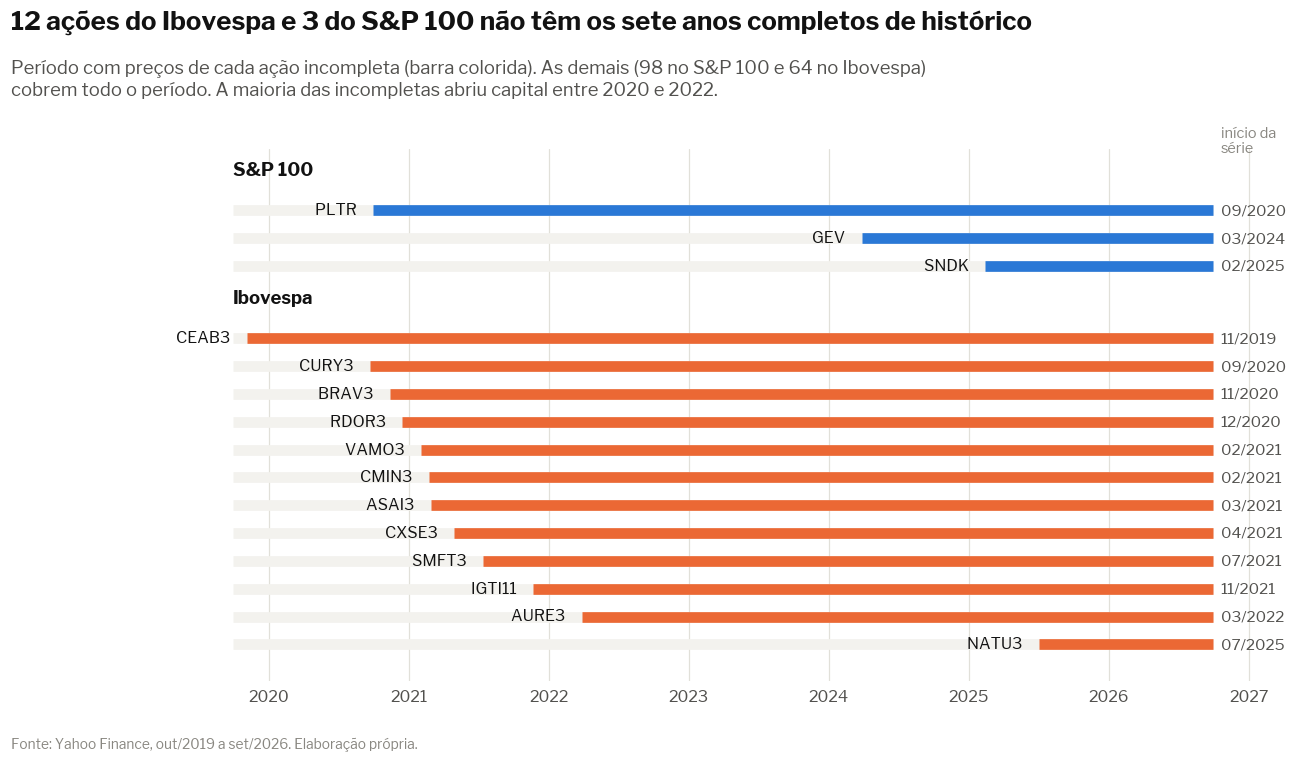
\includegraphics[width=0.92\textwidth]{figures/01_cobertura_dados.png}
    \caption{\textbf{Completude Histórica das Ações dos Universos S\&P 100 e Ibovespa (2019 a 2026).}
    \textbf{Como ler este gráfico:} Cada linha horizontal colorida representa uma ação cujo histórico de preços é incompleto no período de 7 anos. A extensão da barra indica o período em que a ação esteve listada e em negociação efetiva; as datas à direita assinalam o início da série de cotações. As ações omitidas possuem 100\% de completude temporal (98 no S\&P 100 e 64 no Ibovespa).
    \textbf{Interpretação Econômica:} No mercado norte-americano, a quase totalidade das ações (97\%) cobre o período inteiro, com exceções pontuais de cisões ou listagens recentes (SanDisk, GE Vernova e Palantir). No mercado brasileiro, 12 das 76 ações (16\%) possuem histórico truncado, refletindo a grande janela de IPOs ocorrida na B3 entre 2020 e 2021 (ex.: Assaí, Rede D'Or, CSN Mineração). Isso evidencia que o Ibovespa de 2026 possui composição estrutural marcadamente diferente da de 2019.}
    \label{fig:cobertura_dados}
\end{figure}

% ==============================================================================
\section{O Problema de Index Tracking e Relações Euclidianas}
% ==============================================================================

\subsection{Formulação Matemática Canônica}
O objetivo clássico do modelo de \textit{Index Tracking} com restrição de cardinalidade, formulado pioneiramente na literatura de otimização financeira por Cornu{\'e}jols e T{\"u}t{\"u}nc{\"u}~\cite{cornuejols2006optimization}, Beasley et al.~\cite{beasley2003evolutionary} e expandido no mercado brasileiro por Sant'Anna, Filomena e Borenstein~\cite{santanna2014index, santanna2017hybrid}, baseia-se na teoria moderna de carteiras de Markowitz~\cite{markowitz1952portfolio} e na análise de erro de rastreamento de Roll~\cite{roll1992mean}. 

O modelo busca determinar um vetor de pesos $w = (w_1, \dots, w_N)^T$ e um vetor de decisão binária $z = (z_1, \dots, z_N)^T$ que minimizem a distância quadrática média entre o retorno diário da carteira e o do benchmark no período de calibração $t = 1, \dots, T$:

\begin{equation}
\min_{w, z} \; \frac{1}{T} \sum_{t=1}^T \left( R_t - \sum_{i \in I} w_i r_{t,i} \right)^2
\label{eq:miqp_puro}
\end{equation}

\noindent sujeito a:
\begin{align}
\sum_{i \in I} w_i &= 1 \quad &\text{(Orçamento 100\% investido)} \\
w_i &\ge 0 \quad \forall i \in I \quad &\text{(Venda a descoberto proibida / Long-only)} \\
w_i &\le z_i \quad \forall i \in I \quad &\text{(Acoplamento peso-seleção)} \\
\sum_{i \in I} z_i &\le K \quad &\text{(Restrição de cardinalidade máxima de } K \text{ ações)} \\
z_i &\in \{0, 1\} \quad \forall i \in I \quad &\text{(Decisão booleana de inclusão)}
\end{align}

Essa estrutura classifica-se como uma Programação Quadrática Inteira Mista (MIQP). A restrição de cardinalidade $\sum z_i \le K$ converte a regressão linear padrão em um problema combinatório NP-difícil: selecionar $K = 10$ ativos em um universo de $N = 100$ oferece $\binom{100}{10} \approx 1,73 \times 10^{13}$ combinações possíveis, impossibilitando a busca exaustiva por força bruta. Conforme as metodologias oficiais da B3~\cite{b3_ibov_metodologia} e da S\&P Dow Jones Indices~\cite{sp_dow_jones_indices}, a replicação direta de todos os componentes de um índice impõe custos operacionais proibitivos em rebalanceamentos trimestrais.

\subsection{Relação Euclidiana entre RMSE, Tracking Error e Viés}
A função de perda minimizada pelo solver é o Erro Quadrático Médio diário ($\text{MSE}_{\text{diário}}$), cuja raiz quadrada é o $\text{RMSE}_{\text{diário}}$. Seja o resíduo no pregão $t$:
\begin{equation}
e_t = \sum_{i \in I} w_i r_{t,i} - R_t
\end{equation}

A média amostral desse erro (o viés diário) é $\bar{e} = \frac{1}{T} \sum_{t=1}^T e_t$. Reescrevendo $e_t = (e_t - \bar{e}) + \bar{e}$ e calculando a média dos quadrados:
\begin{equation}
\text{MSE}_{\text{diário}} = \frac{1}{T} \sum_{t=1}^T e_t^2 = \frac{1}{T} \sum_{t=1}^T (e_t - \bar{e})^2 + \bar{e}^2 = s_e^2 + \bar{e}^2
\end{equation}

\noindent onde $s_e^2$ é a variância amostral diária dos desvios. Em finanças quantitativas, a anualização obedece a duas convenções distintas de escala temporal:
\begin{enumerate}
    \item \textbf{A tendência/viés acumula-se linearmente no tempo:} $\text{Viés} = 252 \cdot \bar{e} \implies \bar{e} = \frac{\text{Viés}}{252}$.
    \item \textbf{A volatilidade dos erros escala com a raiz do tempo:} $\text{TE} = s_e \sqrt{252} \implies s_e^2 = \frac{\text{TE}^2}{252}$.
    \item \textbf{O RMSE anualizado segue a métrica de volatilidade:} $\text{RMSE}_{\text{anual}}^2 = 252 \cdot \text{MSE}_{\text{diário}}$.
\end{enumerate}

Multiplicando a equação diária por 252 e substituindo os termos:
\begin{equation}
\text{RMSE}_{\text{anual}}^2 = 252 \cdot \left[ \frac{\text{TE}^2}{252} + \left(\frac{\text{Viés}}{252}\right)^2 \right] \implies \mathbf{\text{RMSE}_{\text{anual}}^2 = \text{TE}^2 + \frac{\text{Viés}^2}{252}}
\end{equation}

\paragraph{Geometria no $\mathbb{R}^T$ e o Fator de Bessel:}
No espaço vetorial $\mathbb{R}^T$, o vetor de erros $\mathbf{e}$ decompõe-se ortogonalmente em $\mathbf{e} = \mathbf{e}_{\parallel} + \mathbf{e}_{\perp}$, onde $\mathbf{e}_{\parallel} = \bar{e}\mathbf{1}$ é paralelo ao vetor constante $\mathbf{1} = (1, \dots, 1)^T$ e $\mathbf{e}_{\perp} = \mathbf{e} - \bar{e}\mathbf{1}$ é ortogonal a ele:
\begin{equation}
\langle \mathbf{e}_{\parallel}, \mathbf{e}_{\perp} \rangle = \bar{e} \sum_{t=1}^T (e_t - \bar{e}) = \bar{e}(T\bar{e} - T\bar{e}) = 0
\end{equation}

Pelo Teorema de Pitágoras, $\|\mathbf{e}\|^2 = \|\mathbf{e}_{\parallel}\|^2 + \|\mathbf{e}_{\perp}\|^2$. Além disso, quando calculamos o TE via biblioteca estatística (\texttt{pandas.std}), utiliza-se o estimador não-viesado com $N-1$ graus de liberdade ($ddof=1$), enquanto a média quadrática do MSE divide por $N$ ($ddof=0$). Em uma amostra de $N = 1.242$ pregões de teste (5 anos), o fator de correção é $\sqrt{\frac{N-1}{N}} = \sqrt{\frac{1241}{1242}} \approx 0,9996$, reconciliando o cálculo até a sexta casa decimal.

% ==============================================================================
\section{Coleta, Integridade e Auditoria de Dados}
% ==============================================================================

\subsection{Convenções de Preços e Calendários}
Coletamos cotações diárias de 30/09/2019 a 30/09/2026 (1.759 pregões no S\&P 100 e 1.742 no Ibovespa). Cada mercado adota a convenção metodológica do seu benchmark:
\begin{itemize}
    \item \textbf{S\&P 100 (\texttt{\^{}OEX}):} Índice de retorno de preços (\textit{price return}). Desconsidera o pagamento de dividendos. As ações utilizam preço de fechamento bruto (\texttt{Close}).
    \item \textbf{IBOVESPA (\texttt{\^{}BVSP}):} Índice de retorno total (\textit{total return}). Reinveste automaticamente todos os proventos brutos. As ações utilizam o fechamento ajustado (\texttt{Adj Close}).
\end{itemize}

\subsection{Triagem Algorítmica e Auditoria Oficial}
Submetemos os 302.041 retornos diários a três filtros estatísticos de consistência:
\begin{enumerate}
    \item \textbf{Salto Isolado:} Variação diária $\ge 40\%$ com o índice variando menos de $2\%$.
    \item \textbf{Salto que se Desfaz:} Variação $\ge 10\%$ devolvida em pelo menos $80\%$ no pregão seguinte, com mercado estável.
    \item \textbf{Salto no Fator de Ajuste:} Razão $\text{Adj Close}/\text{Close}$ oscilando mais de $25\%$ em um único dia.
\end{enumerate}

\begin{figure}[H]
    \centering
    \begin{subfigure}[b]{0.48\textwidth}
        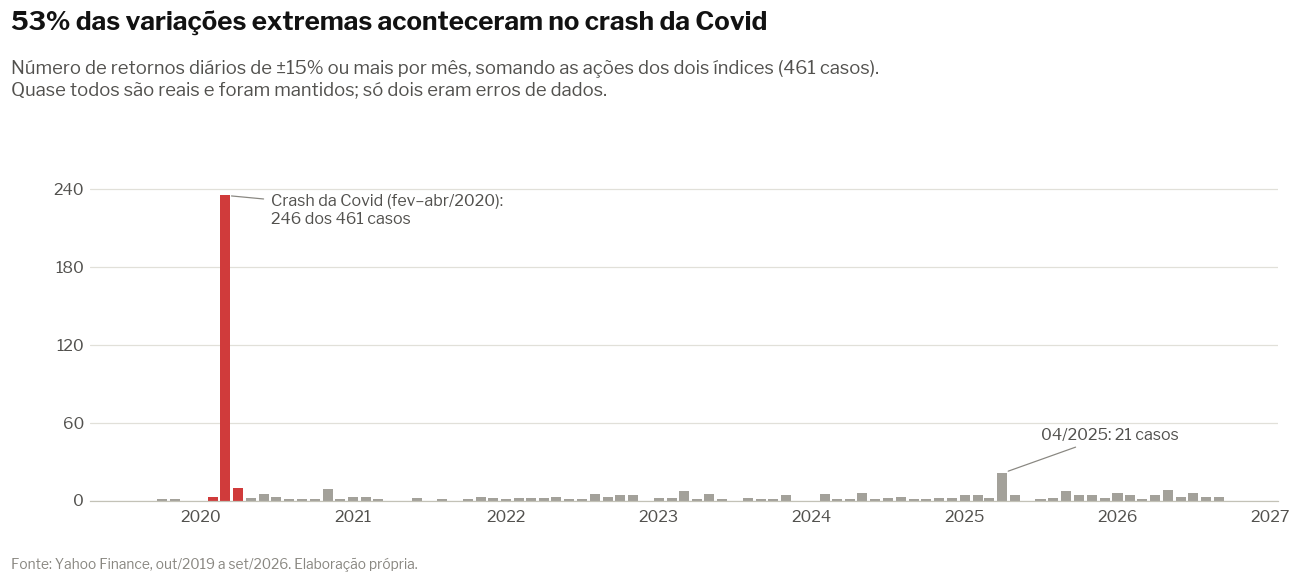
\includegraphics[width=\textwidth]{figures/01b_outliers_por_mes.png}
        \caption{Distribuição temporal dos 460 retornos extremos.}
    \end{subfigure}
    \hfill
    \begin{subfigure}[b]{0.48\textwidth}
        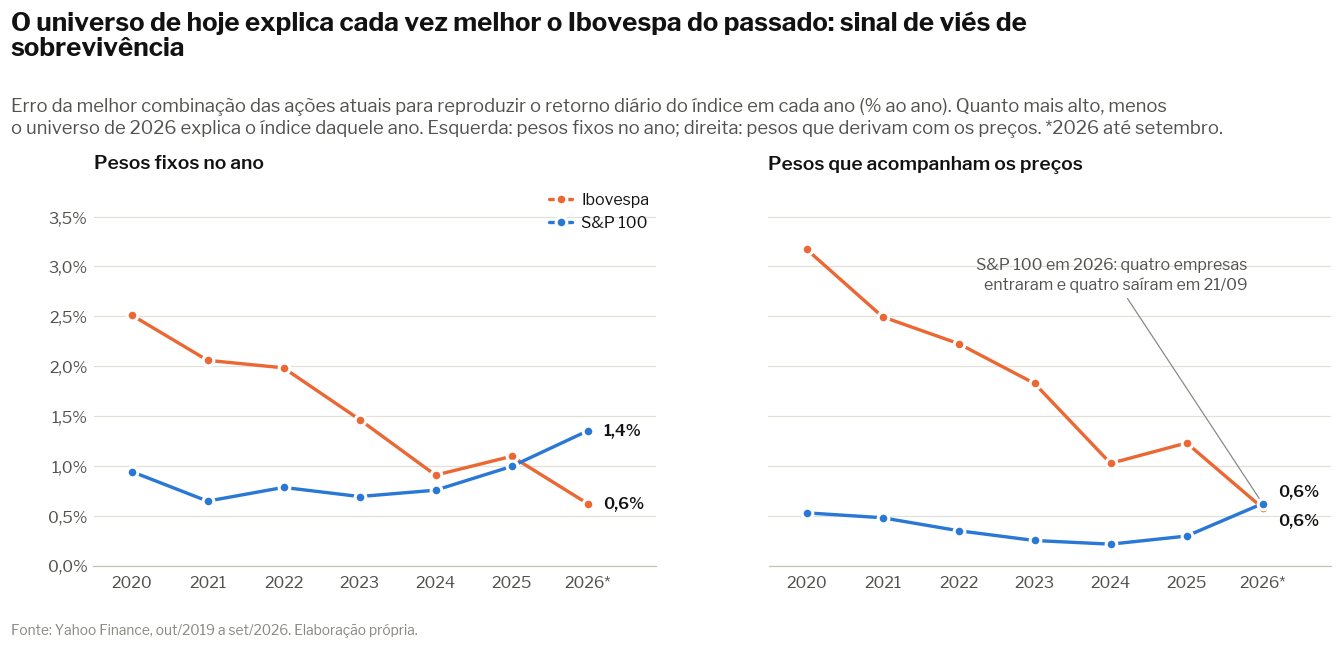
\includegraphics[width=\textwidth]{figures/12_consistencia_universo_indice.png}
        \caption{Erro residual do universo de 2026 explicando o passado.}
    \end{subfigure}
    \caption{\textbf{Diagnósticos de Integridade: Distribuição de Extremos e Consistência Temporal.}
    \textbf{Como ler este gráfico:} À esquerda (a), as barras verticais mostram a contagem de retornos diários absolutos $\ge 15\%$ por mês, evidenciando o choque concentrado de março/2020 (crash da Covid-19, com 246 casos). À direita (b), traça-se o Tracking Error residual ótimo da carteira formada por todas as ações disponíveis em 2026 para replicar o índice ano a ano. A linha azul representa o S\&P 100 e a linha laranja o Ibovespa.
    \textbf{Interpretação Econômica:} O gráfico (b) evidencia a magnitude do viés de sobrevivência: quanto mais recuamos no tempo, pior o universo de ações de 2026 explica o Ibovespa (o erro residual sobe de 0,6\% em 2026 para 3,2\% em 2020 com pesos que derivam com os preços). Isso ocorre porque empresas relevantes da época saíram do índice ou foram incorporadas, demonstrando a importância de controlar o viés Point-in-Time.}
    \label{fig:extremos_consistencia}
\end{figure}

A conferência na base oficial da B3 (COTAHIST) confirmou dois erros reais do provedor público:
\begin{itemize}
    \item \textbf{Ultrapar (\texttt{UGPA3}) em 28/06/2021:} O fechamento bruto saltava de R\$ 8,75 para R\$ 19,19 (+119\%). A cotação oficial da B3 registrou R\$ 18,99 e R\$ 19,19 (+1,05\%). A série histórica do Yahoo estava descalibrada em escala 2,2x. A série foi reescalada e o retorno corrigido.
    \item \textbf{Copasa (\texttt{CSMG3}) em 19/11/2020:} O Yahoo descontou um dividendo extraordinário de R\$ 6,49 um pregão antes da data-ex oficial, gerando salto de +16,9\% e queda de -12,4\%. Ambas as cotações foram substituídas pelas oficiais.
\end{itemize}

% ==============================================================================
\section{Análise Exploratória e Estrutura de Mercado}
% ==============================================================================

\subsection{Comportamento Histórico, Rentabilidade e Retornos Anuais}
Em sete anos, o S\&P 100 acumulou alta de $+190,7\%$ (em USD), impulsionado pelas empresas de semicondutores e tecnologia, enquanto o Ibovespa valorizou $+77,9\%$ (em BRL). Os retornos diários violam fortemente a hipótese de normalidade gaussiana, apresentando curtose excessiva acentuada (13,1 no S\&P e 20,7 no Ibovespa).

\begin{figure}[H]
    \centering
    \begin{subfigure}[b]{0.48\textwidth}
        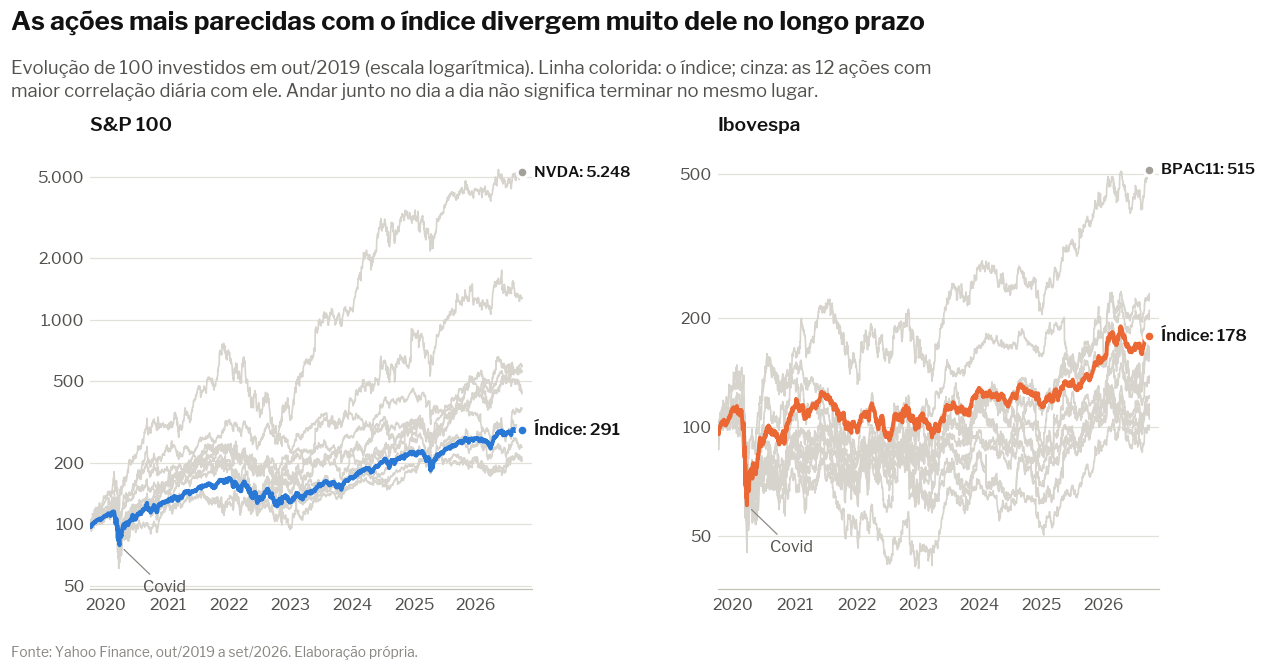
\includegraphics[width=\textwidth]{figures/02_performance.png}
        \caption{Evolução acumulada (Base 100 = 2019).}
    \end{subfigure}
    \hfill
    \begin{subfigure}[b]{0.48\textwidth}
        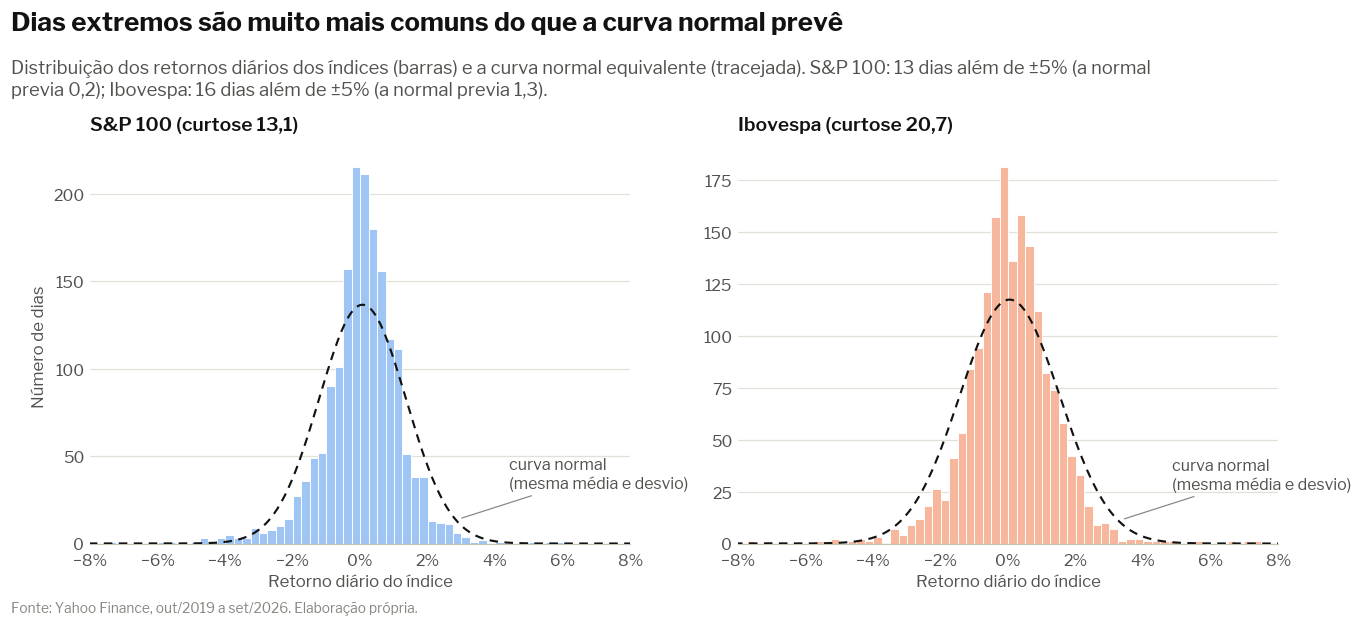
\includegraphics[width=\textwidth]{figures/02b_distribuicao_retornos.png}
        \caption{Histograma vs. Distribuição Gaussiana.}
    \end{subfigure}
    \caption{\textbf{Desempenho Acumulado dos Índices e Evidência Empírica de Caudas Gordas.}
    \textbf{Como ler este gráfico:} Em (a), exibe-se a evolução patrimonial de 100 investidos em outubro/2019 na linha azul (S\&P 100) e laranja (Ibovespa), com as 12 ações mais correlacionadas representadas em cinza de fundo em escala logarítmica. Em (b), as barras indicam a densidade empírica dos retornos diários dos benchmarks frente à curva normal teórica (linha tracejada preta) ajustada com a mesma média e desvio-padrão.
    \textbf{Interpretação Econômica:} As ações individuais apresentam dispersão astronômica no longo prazo: a Nvidia multiplicou seu valor por mais de 50 vezes, enquanto ativos deprimidos caíram mais de 60\%. No painel (b), a presença de caudas gordas (\textit{fat tails}) comprova que choques diários superiores a $\pm 5\%$ ocorrem com frequência ordens de grandeza superior à prevista pelo modelo normal, justificando por que a minimização quadrática de erros é sensível a choques de volatilidade.}
    \label{fig:performance_fat_tails}
\end{figure}

\begin{figure}[H]
    \centering
    \begin{subfigure}[b]{0.48\textwidth}
        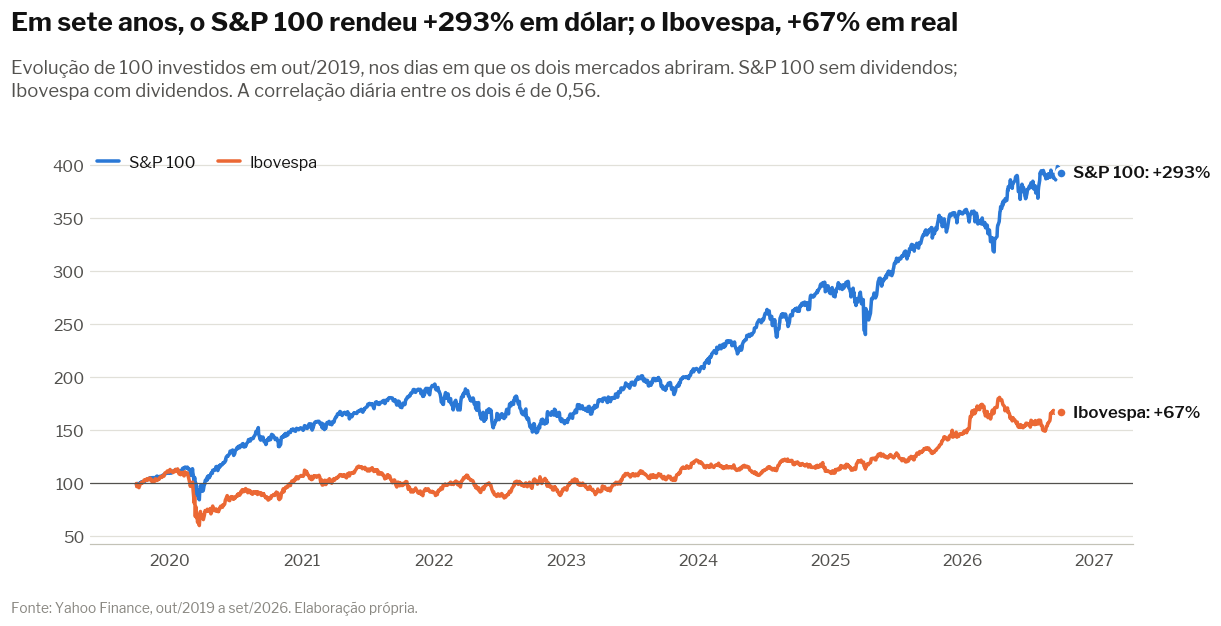
\includegraphics[width=\textwidth]{figures/04_comparacao_benchmarks.png}
        \caption{Evolução acumulada comparativa dos benchmarks.}
    \end{subfigure}
    \hfill
    \begin{subfigure}[b]{0.48\textwidth}
        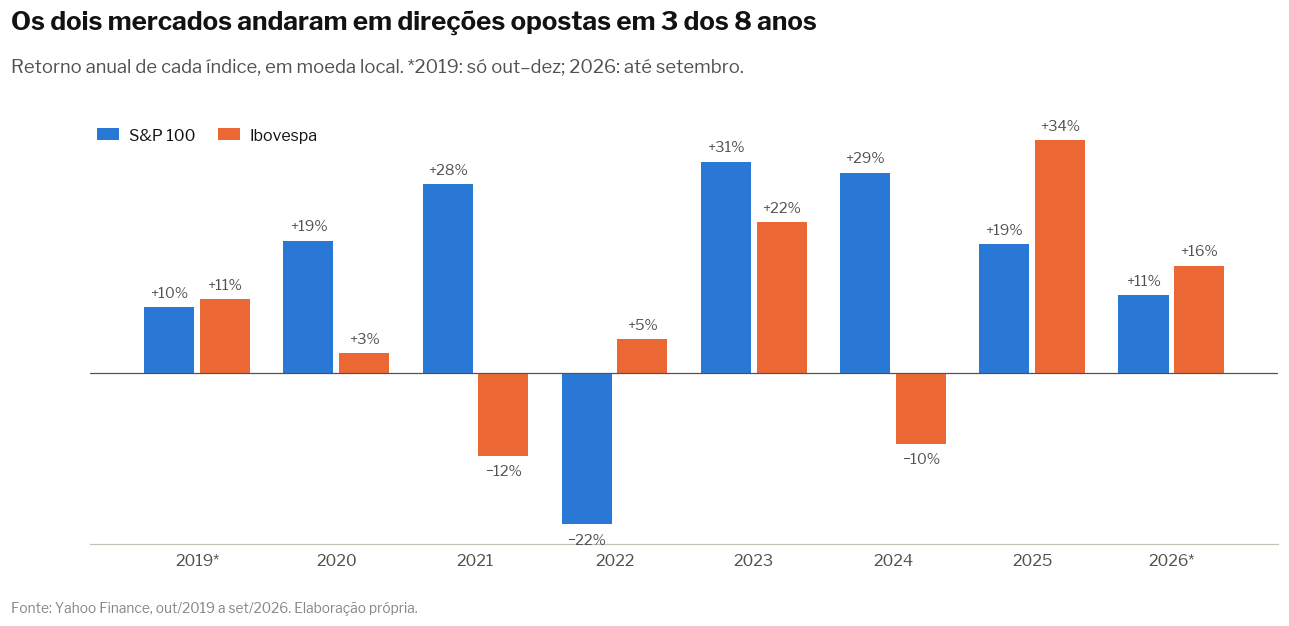
\includegraphics[width=\textwidth]{figures/04b_retornos_anuais.png}
        \caption{Retornos anuais comparativos por ano civil.}
    \end{subfigure}
    \caption{\textbf{Comparação Direta de Rentabilidade e Divergência Anual entre S\&P 100 e Ibovespa.}
    \textbf{Como ler este gráfico:} Em (a), as trajetórias patrimoniais normalizadas em 100 em 2019 ilustram o descolamento de longo prazo entre os mercados. Em (b), as barras horizontais comparam os retornos anuais consolidados em moeda local.
    \textbf{Interpretação Econômica:} Os dois mercados andaram em direções opostas em 3 dos 6 anos completos analisados (2021, 2022 e 2024). Enquanto em 2021 o S\&P 100 subiu $+26,4\%$ e o Ibovespa caiu $-11,9\%$, em 2022 a bolsa brasileira avançou $+4,7\%$ e a americana caiu $-19,6\%$. Essa assimetria reflete ciclos monetários e exposições setoriais distintas (commodities no Brasil vs. tecnologia nos EUA).}
    \label{fig:benchmarks_anuais}
\end{figure}

\subsection{Volatilidade Móvel e Regimes Econômicos}
A volatilidade anualizada calculada em janelas móveis de 21 pregões atingiu picos históricos no crash da COVID-19 (95\% a.a. no S\&P 100 e 127\% a.a. no Ibovespa em abril/2020), estabilizando-se em 15\% a 17\% a.a. em períodos de calmaria.

\begin{figure}[H]
    \centering
    \begin{subfigure}[b]{0.48\textwidth}
        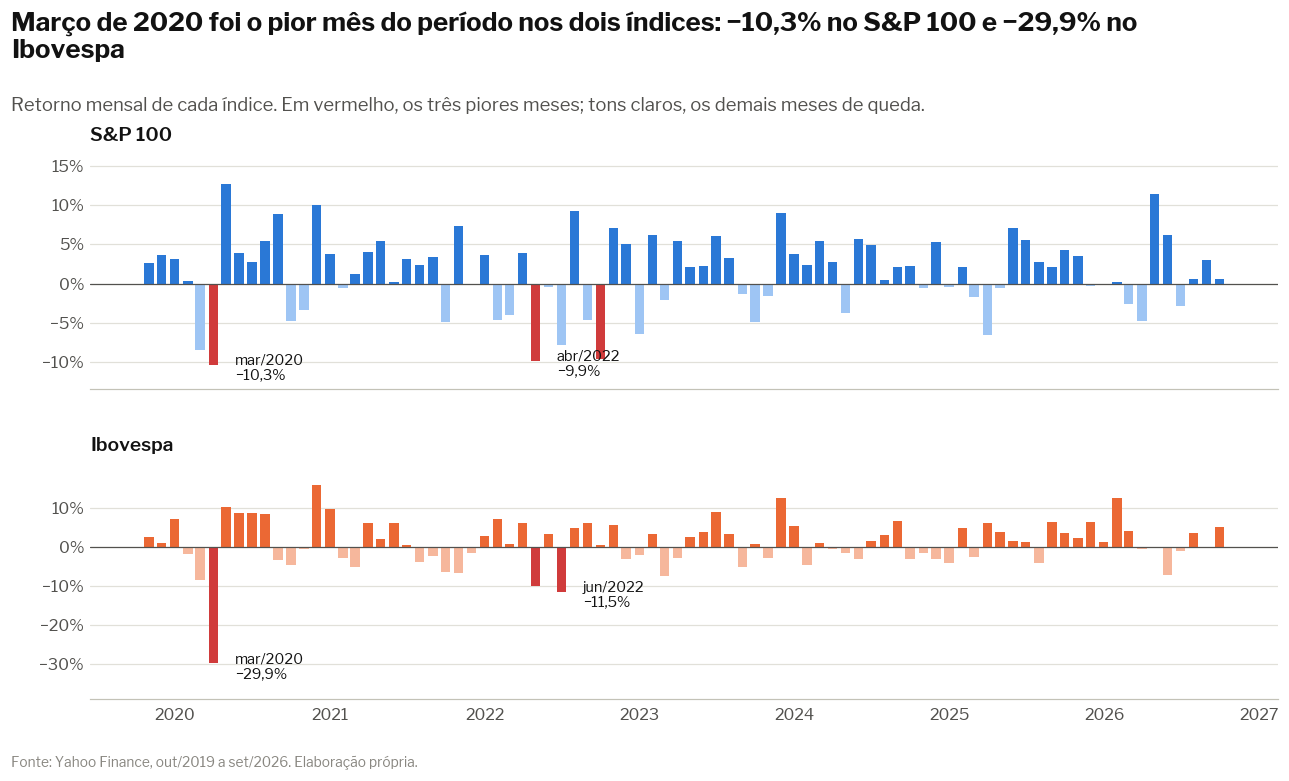
\includegraphics[width=\textwidth]{figures/03_retornos_mensais.png}
        \caption{Distribuição dos retornos mensais dos benchmarks.}
    \end{subfigure}
    \hfill
    \begin{subfigure}[b]{0.48\textwidth}
        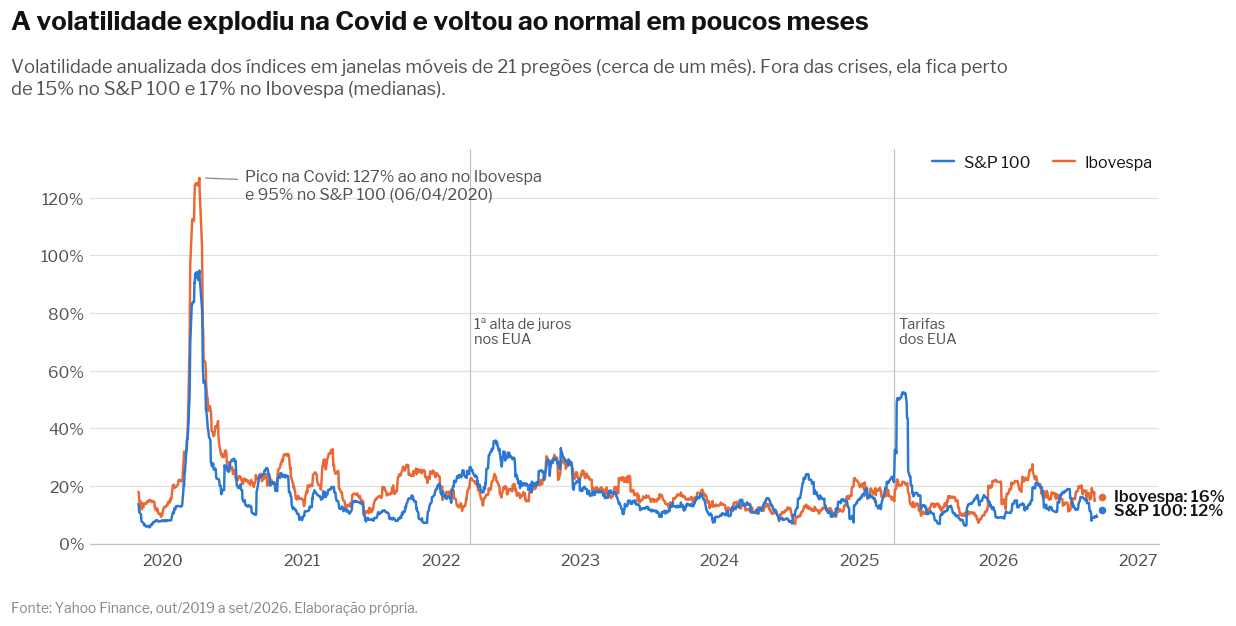
\includegraphics[width=\textwidth]{figures/03b_volatilidade.png}
        \caption{Volatilidade histórica móvel anualizada (21 pregões).}
    \end{subfigure}
    \caption{\textbf{Dinâmica Temporal: Retornos Mensais e Volatilidade Móvel Anualizada (21d).}
    \textbf{Como ler este gráfico:} Em (a), as barras detalham o retorno de cada mês (barras em destaque de alerta para os piores meses da série histórica). Em (b), a linha contínua exibe a volatilidade móvel em janelas de 21 dias úteis (1 mês) com anotações dos eventos de estresse macroeconômico global.
    \textbf{Interpretação Econômica:} Março de 2020 foi o pior mês de toda a amostra em ambos os mercados: $-10,3\%$ no S\&P 100 e $-29,9\%$ no Ibovespa. A volatilidade disparou para $95\%$ a.a. nos EUA e $127\%$ a.a. no Brasil, normalizando-se após 4 meses. Essa dinâmica de \textit{volatility clustering} evidencia que matrizes de covariância calculadas em crises não representam o regime estacionário do mercado.}
    \label{fig:retornos_mensais_vol}
\end{figure}

\subsection{Aderência Individual e Matrizes de Correlação}
A análise de correlação entre os ativos individuais e os índices revela que nenhuma ação sozinha consegue espelhar o mercado, exigindo diversificação ponderada.

\begin{figure}[H]
    \centering
    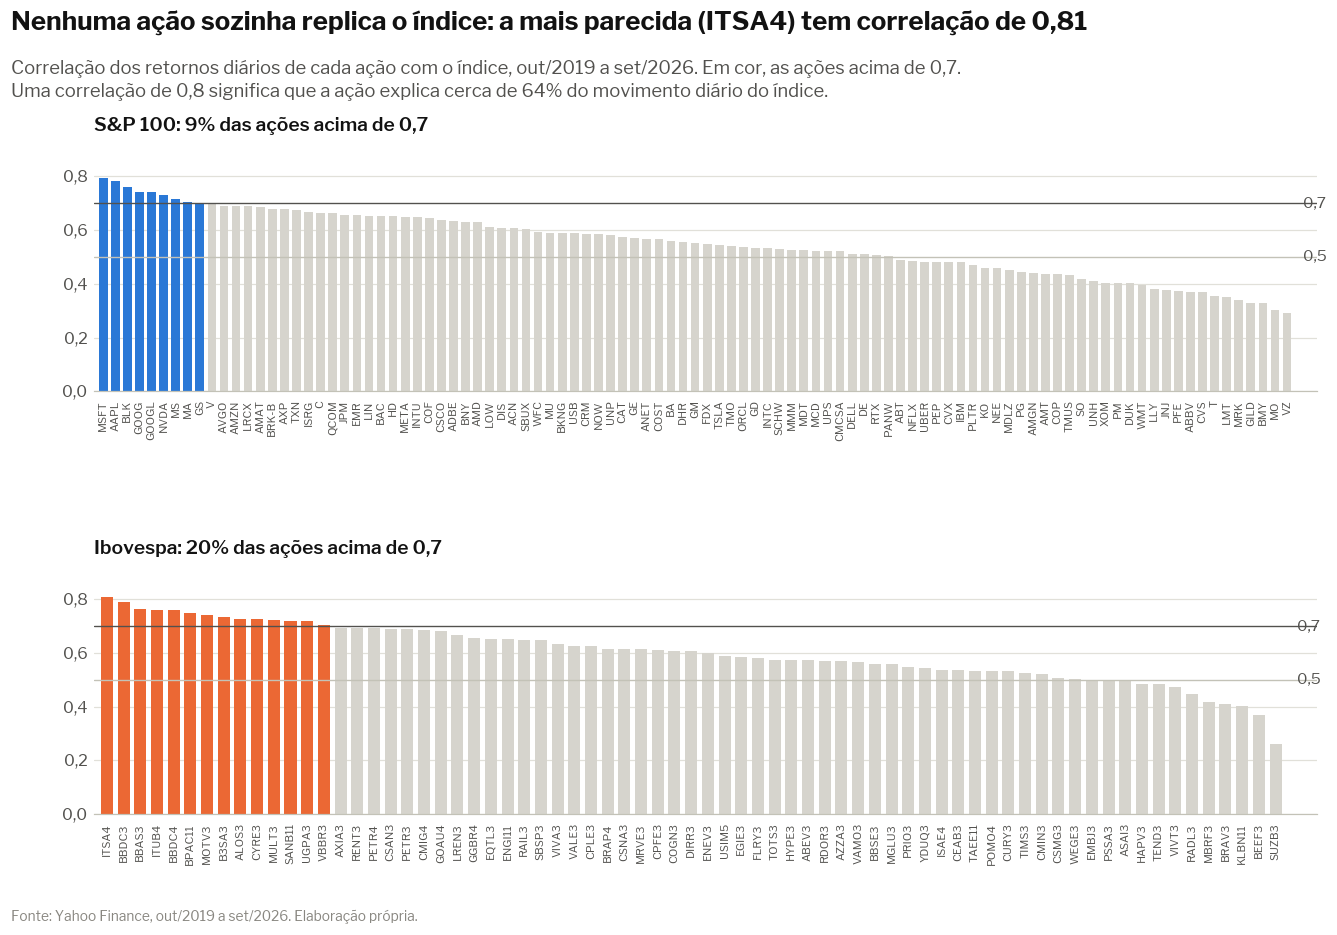
\includegraphics[width=0.92\textwidth]{figures/14_correlacao_com_indice_ranqueada.png}
    \caption{\textbf{Distribuição Ranqueada da Correlação Linear de Todos os Ativos com o Benchmark.}
    \textbf{Como ler este gráfico:} Cada barra vertical representa uma ação individual do universo elegível, ordenada da maior para a menor correlação com o respectivo benchmark ao longo do período completo de 7 anos. As linhas horizontais de referência marcam os limiares de $\rho = 0,50$ e $\rho = 0,70$.
    \textbf{Interpretação Econômica:} Nenhuma ação sozinha é capaz de replicar satisfatoriamente o benchmark. A ação com maior aderência individual atinge $\rho = 0,81$ no S\&P 100 (Microsoft) e $\rho = 0,79$ no Ibovespa (Itaú Unibanco). Mais de $55\%$ das ações do S\&P 100 superam o patamar de correlação de $0,70$, enquanto no Ibovespa apenas $38\%$ atingem essa marca, confirmando maior homogeneidade setorial no mercado americano.}
    \label{fig:correlacao_ranqueada}
\end{figure}

A correlação entre ativos indica alto grau de redundância entre classes de ações da mesma companhia ou holdings controladoras: Alphabet A e C ($\rho = 0,996$), Petrobras ON e PN ($\rho = 0,970$), Bradesco ON e PN ($\rho = 0,970$) e Itaúsa e Itaú ($\rho = 0,920$).

\begin{figure}[H]
    \centering
    \begin{subfigure}[b]{0.48\textwidth}
        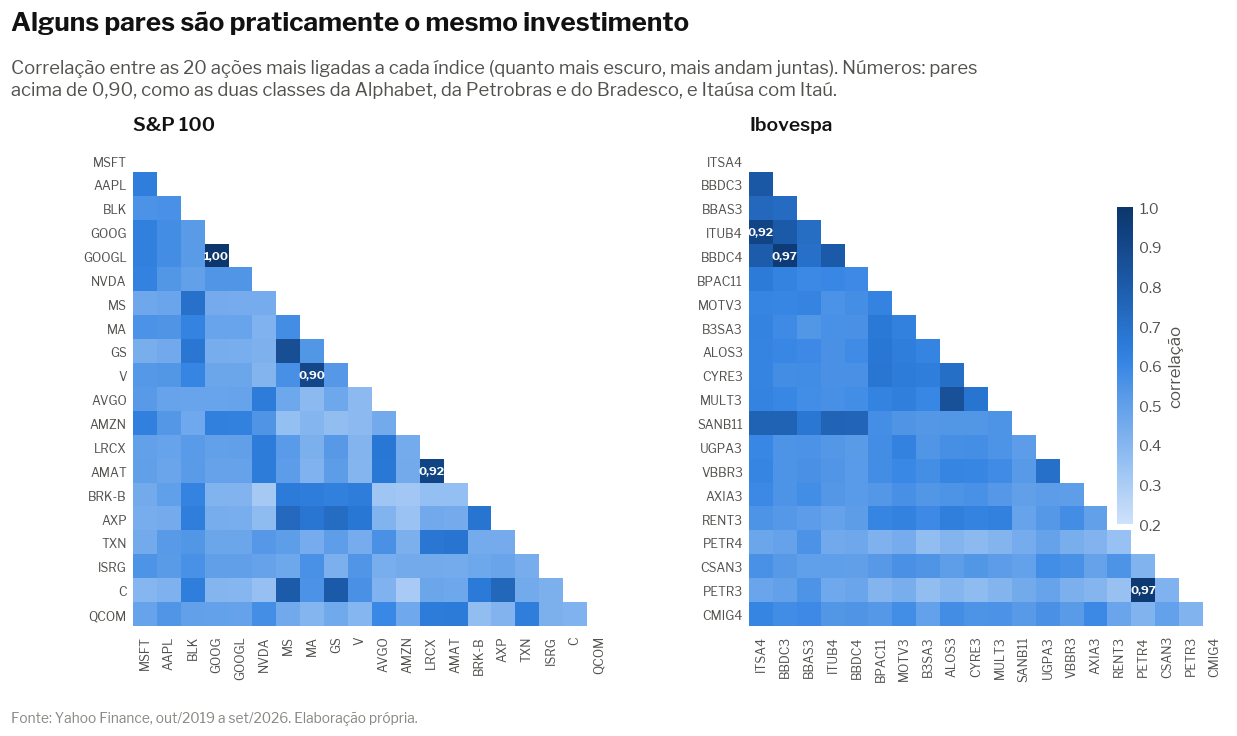
\includegraphics[width=\textwidth]{figures/05_heatmaps_correlacao.png}
        \caption{Pares com redundância estatística ($\rho > 0,90$).}
    \end{subfigure}
    \hfill
    \begin{subfigure}[b]{0.48\textwidth}
        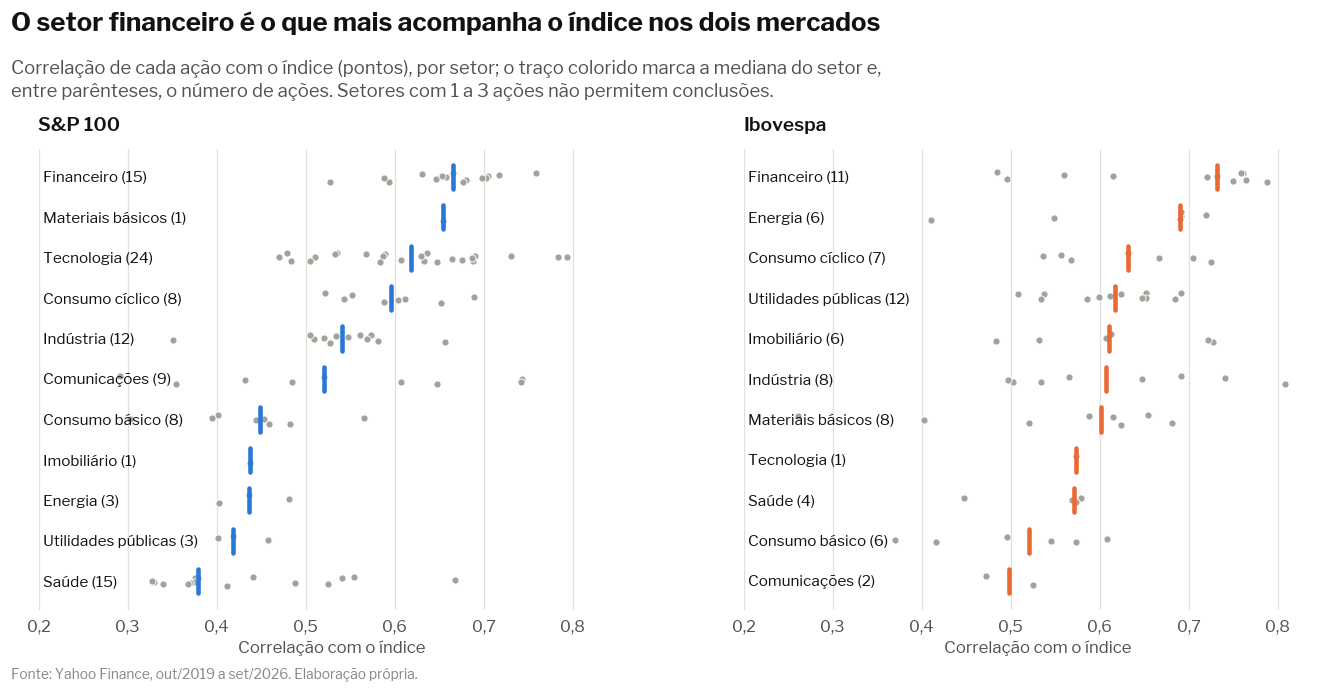
\includegraphics[width=\textwidth]{figures/06_correlacao_por_setor.png}
        \caption{Distribuição da correlação por setor.}
    \end{subfigure}
    \caption{\textbf{Estrutura de Correlação Interativo e Dispersão Setorial.}
    \textbf{Como ler este gráfico:} Em (a), exibe-se a metade inferior da matriz de correlação das 30 ações mais aderentes ao benchmark; tons avermelhados/azulados escuros indicam forte covariância positiva. Em (b), apresentam-se os boxplots da correlação de cada ativo com o benchmark agrupados por setor econômico.
    \textbf{Interpretação Econômica:} O gráfico (a) comprova a existência de ativos duplicados: em uma carteira restrita a $K = 10$, alocar tanto PETR3 quanto PETR4 consome duas vagas sem ganho informacional. Em (b), o setor financeiro destaca-se como o mais aderente ao benchmark nos dois países ($\rho = 0,66$ no S\&P e $\rho = 0,68$ no Ibovespa), enquanto setores defensivos e exportadores (ex.: papel e celulose) possuem baixa correlação com a bolsa local.}
    \label{fig:heatmaps_setores}
\end{figure}

\begin{figure}[H]
    \centering
    \begin{subfigure}[b]{0.48\textwidth}
        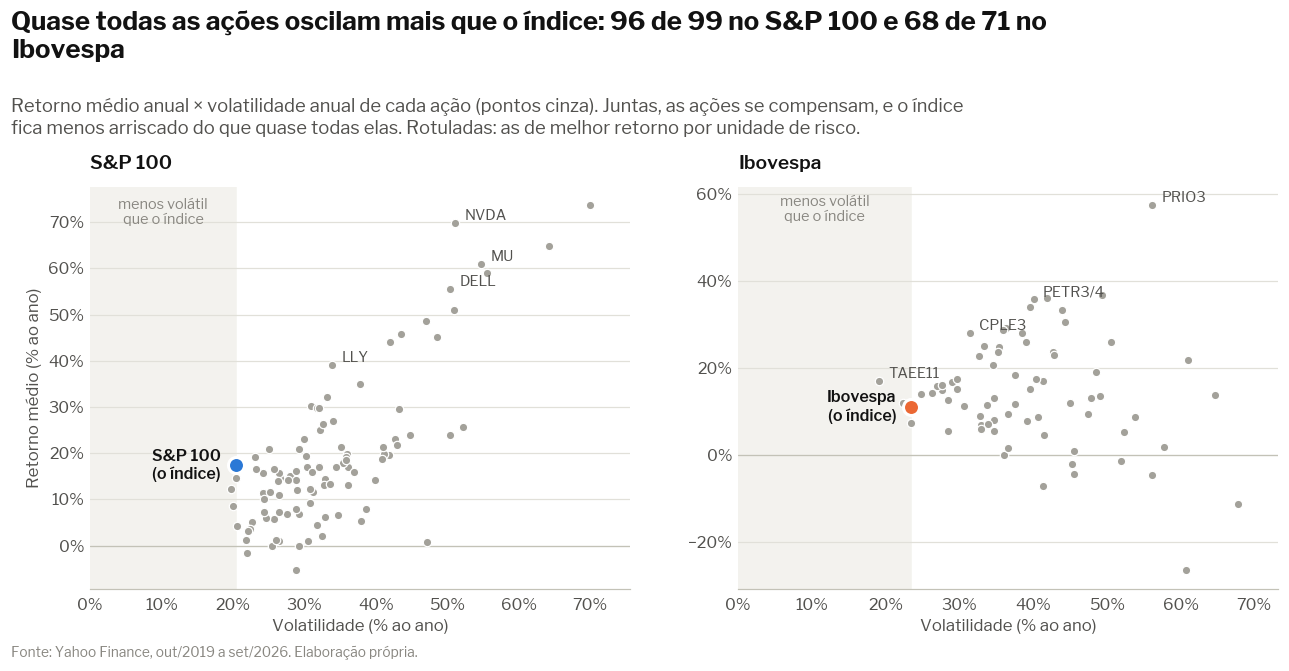
\includegraphics[width=\textwidth]{figures/13_risco_retorno.png}
        \caption{Fronteira de dispersão Risco $\times$ Retorno.}
    \end{subfigure}
    \hfill
    \begin{subfigure}[b]{0.48\textwidth}
        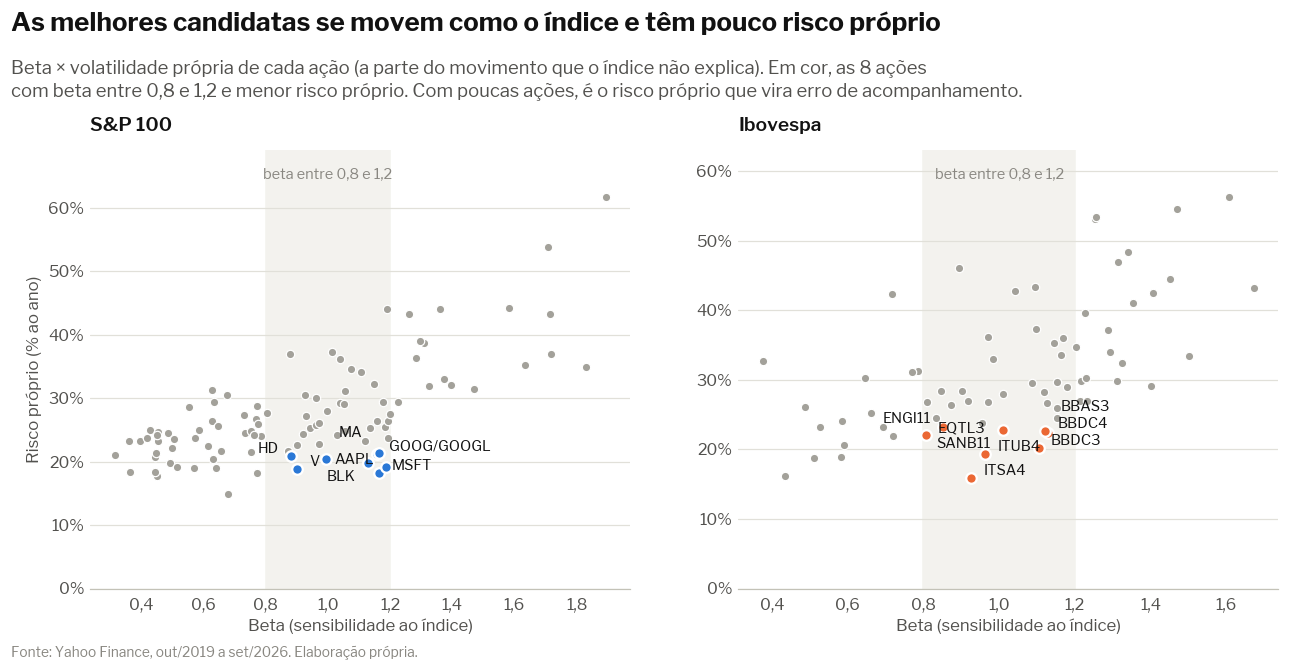
\includegraphics[width=\textwidth]{figures/15_beta_risco_idiossincratico.png}
        \caption{Beta vs. Risco Idiossincrático.}
    \end{subfigure}
    \caption{\textbf{Análise de Risco e Retorno e Decomposição de Risco Idiossincrático.}
    \textbf{Como ler este gráfico:} Em (a), o ponto colorido marca a posição do índice de mercado e os pontos cinzas marcam as ações individuais; a faixa cinza destaca o patamar de volatilidade inferior ao do próprio índice. Em (b), mapeia-se a sensibilidade ao mercado (beta no eixo X) contra a volatilidade do resíduo não explicado pelo índice (risco próprio no eixo Y).
    \textbf{Interpretação Econômica:} O painel (a) demonstra que a diversificação reduz drasticamente o risco: 96 de 99 ações no S\&P e 68 de 71 no Ibov possuem volatilidade superior à do índice. No painel (b), identificam-se as candidatas naturais ao rastreamento passivo: ações que possuem beta unitário ($\beta \in [0,8; 1,2]$) aliado a baixo risco idiossincrático (pontos destacados: Microsoft, Visa, Apple, Itaú e Bradesco).}
    \label{fig:risco_retorno_beta}
\end{figure}

\subsection{Estabilidade Temporal e Liquidez Operacional}
A capacidade de prever pesos ótimos depende da estabilidade temporal dos parâmetros estatísticos e da liquidez de negociação dos papéis.

\begin{figure}[H]
    \centering
    \begin{subfigure}[b]{0.48\textwidth}
        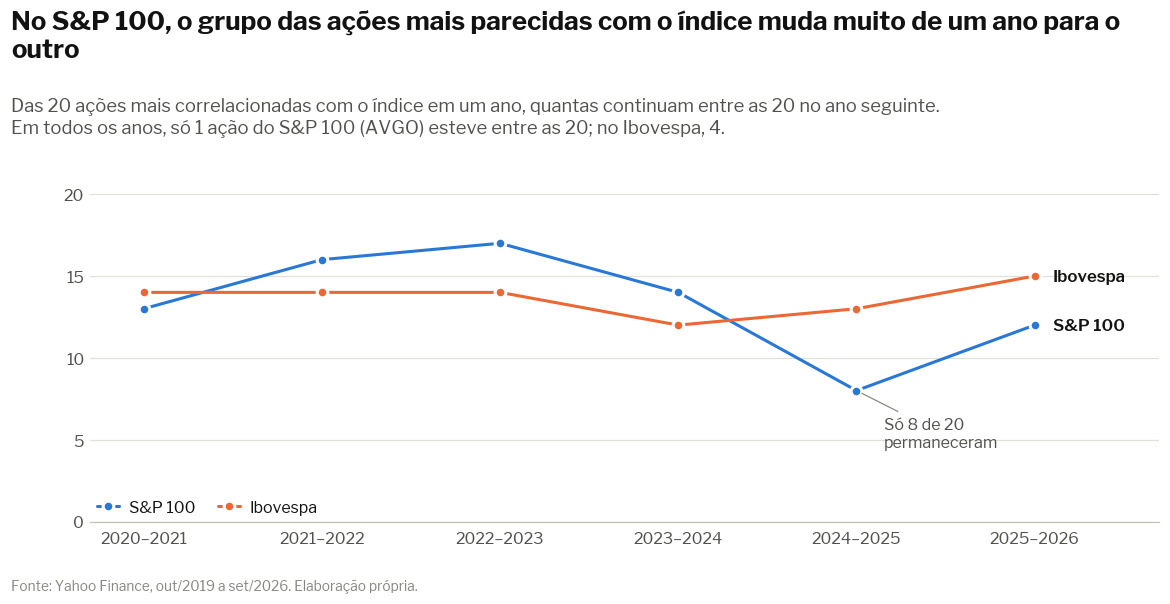
\includegraphics[width=\textwidth]{figures/16_estabilidade_ranking.png}
        \caption{Persistência anual do Top 20 de correlação.}
    \end{subfigure}
    \hfill
    \begin{subfigure}[b]{0.48\textwidth}
        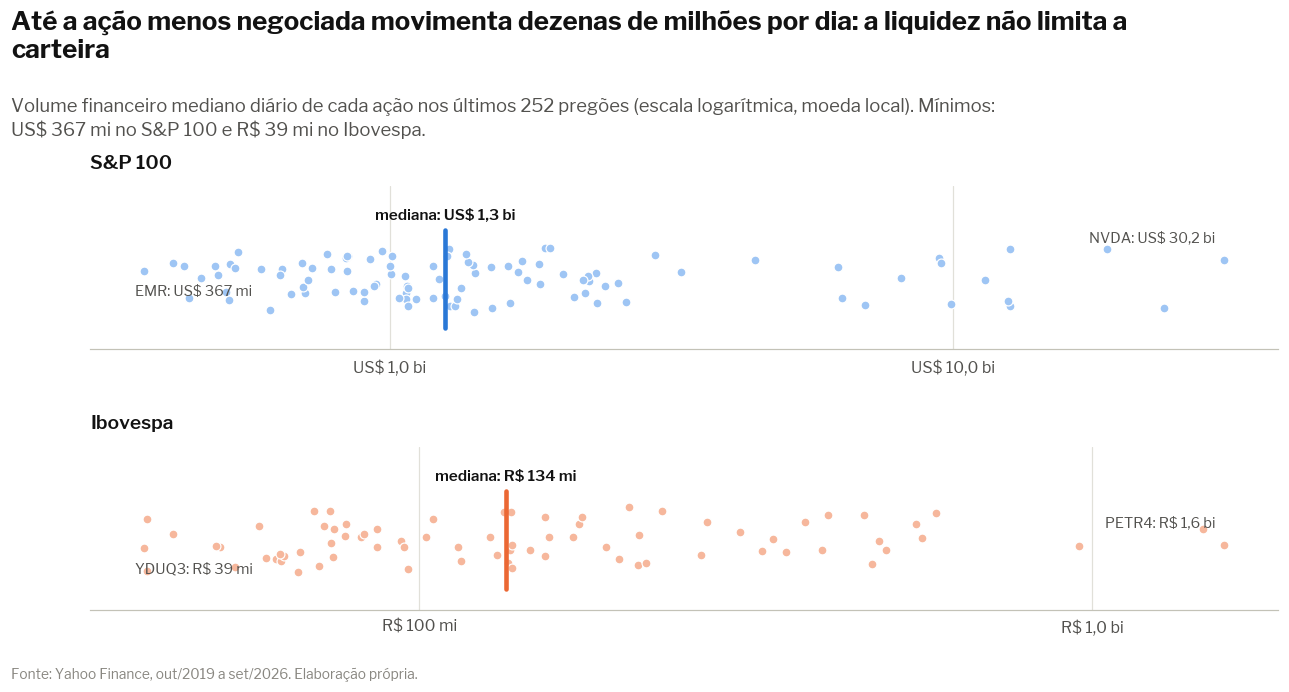
\includegraphics[width=\textwidth]{figures/19_liquidez.png}
        \caption{Liquidez mediana diária e dias com retorno zero.}
    \end{subfigure}
    \caption{\textbf{Estabilidade Temporal dos Ativos Candidatos e Perfil de Liquidez de Mercado.}
    \textbf{Como ler este gráfico:} Em (a), mede-se a quantidade de ações que permanecem no grupo das 20 maiores correlações na transição entre anos consecutivos. Em (b), mapeia-se o volume financeiro mediano diário (em escala logarítmica) contra a porcentagem de dias sem retorno (dias com retorno zero).
    \textbf{Interpretação Econômica:} O painel (a) revela que a correlação não é um fator estável no tempo: na virada de 2021 para 2022, apenas 9 das 20 ações permaneceram no topo do ranking no S\&P 100. Isso explica a fragilidade da heurística de seleção prévia por correlação. No painel (b), comprova-se que a liquidez não limita o modelo: até a ação menos negociada movimenta dezenas de milhões de reais por dia na B3 e mais de US\$ 80 milhões no S\&P 100, com zero dias de iliquidez severa.}
    \label{fig:estabilidade_liquidez}
\end{figure}

\subsection{A Descoberta Central da Estrutura de Mercado: O Descolamento Pós-2023}
Avaliando a coesão média entre pares de ativos ao longo do tempo (janelas móveis de 63 pregões), identificamos que o S\&P 100 sofreu um descolamento histórico a partir de 2023: sua correlação média caiu para 0,19, enquanto o Ibovespa permaneceu coeso ($\rho \approx 0,33$). 

\begin{figure}[H]
    \centering
    \begin{subfigure}[b]{0.48\textwidth}
        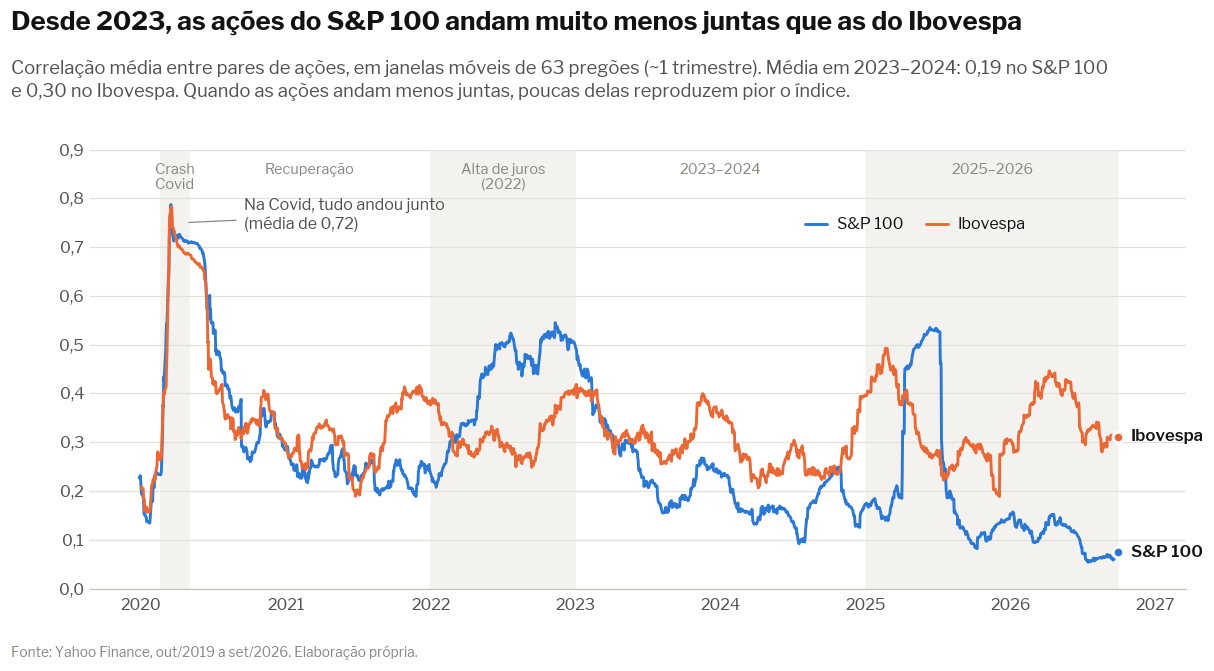
\includegraphics[width=\textwidth]{figures/11_correlacao_por_regime.png}
        \caption{Coesão média móvel entre ações (63d).}
    \end{subfigure}
    \hfill
    \begin{subfigure}[b]{0.48\textwidth}
        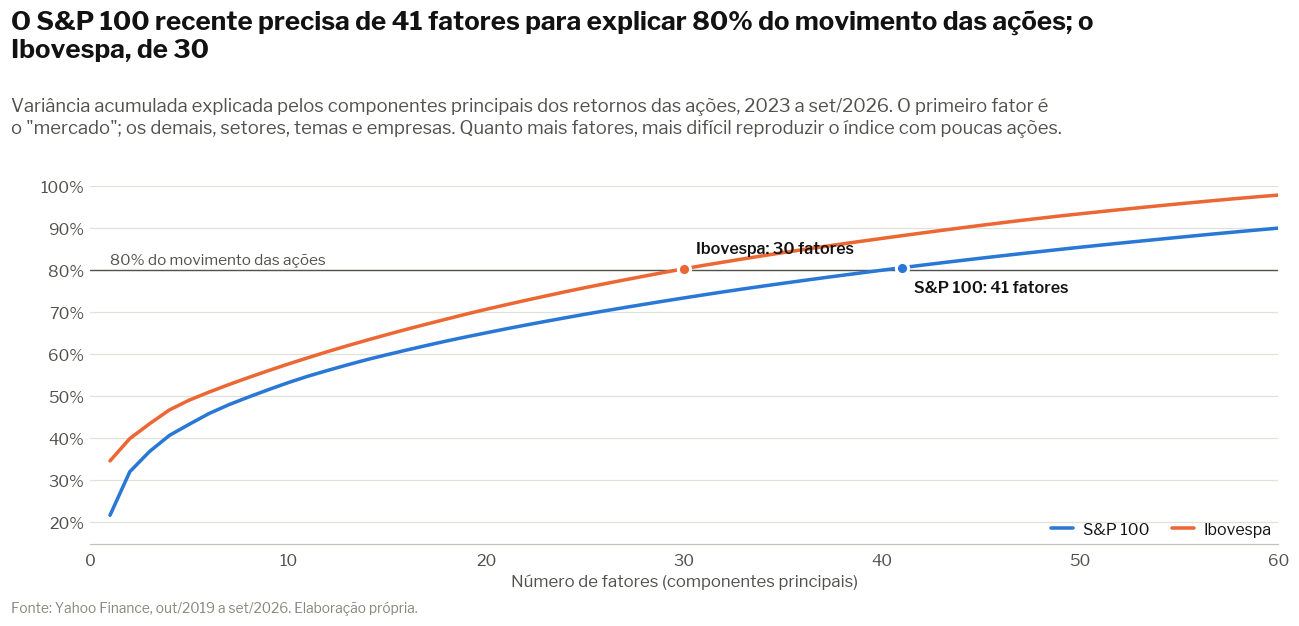
\includegraphics[width=\textwidth]{figures/18_pca_variancia_acumulada.png}
        \caption{Variância acumulada via PCA.}
    \end{subfigure}
    \caption{\textbf{A Descoberta Central: Descolamento do S\&P 100 e Fatores de Variância.}
    \textbf{Como ler este gráfico:} Em (a), traça-se a correlação média de todos os pares possíveis de ações ao longo do tempo para o S\&P 100 (linha azul) e Ibovespa (linha laranja). Em (b), exibe-se a fração de variância total explicada pelo número acumulado de componentes principais (PCA) no período recente (2023–2026).
    \textbf{Interpretação Econômica:} O painel (a) revela que na crise da COVID o mercado inteiro se moveu em bloco ($\rho \approx 0,72$). A partir de 2023, o rali concentrado em IA causou dispersão extrema no mercado norte-americano. Consequentemente, o gráfico (b) comprova matematicamente por que o S\&P 100 tornou-se mais difícil de replicar com poucas ações do que o Ibovespa: são necessários 41 fatores para cobrir 80\% da variância do S\&P recente, contra 30 fatores no Ibovespa.}
    \label{fig:descolamento_pca}
\end{figure}

\begin{figure}[H]
    \centering
    \begin{subfigure}[b]{0.48\textwidth}
        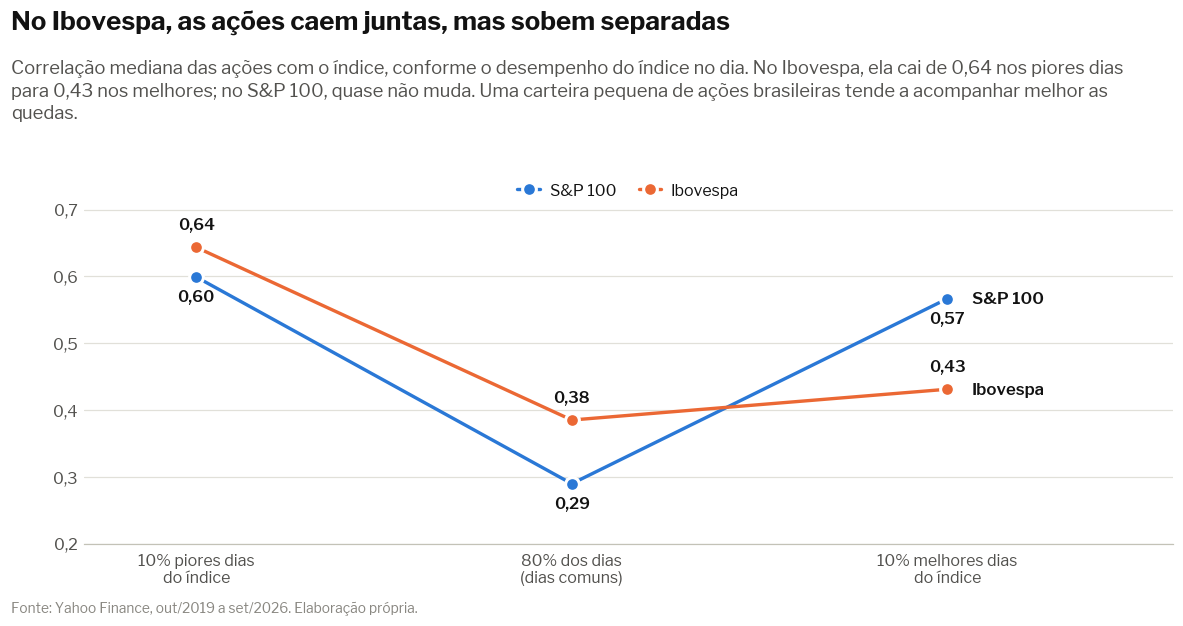
\includegraphics[width=\textwidth]{figures/17_assimetria_correlacao.png}
        \caption{Assimetria de correlação por regime de retorno.}
    \end{subfigure}
    \hfill
    \begin{subfigure}[b]{0.48\textwidth}
        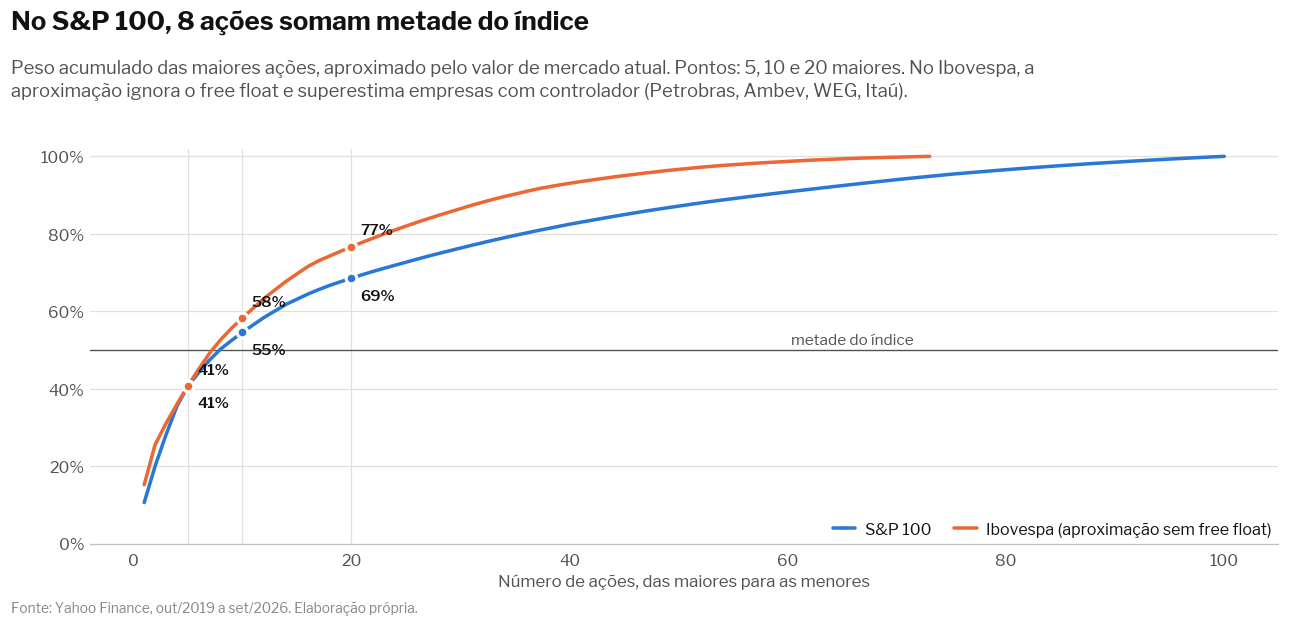
\includegraphics[width=\textwidth]{figures/20_concentracao_indices.png}
        \caption{Curva de concentração de peso acumulado.}
    \end{subfigure}
    \caption{\textbf{Assimetria de Cauda no Brasil e Concentração de Peso nos Benchmarks.}
    \textbf{Como ler este gráfico:} Em (a), mede-se a correlação típica das ações com o benchmark segregada entre os 10\% piores dias, 80\% centrais e 10\% melhores dias do índice. Em (b), traça-se a curva de peso acumulado das maiores companhias por valor de mercado.
    \textbf{Interpretação Econômica:} O painel (a) comprova a assimetria estrutural da B3: nos dias de pânico, a correlação das ações brasileiras salta para 0,64, enquanto nos dias de forte alta cai para 0,43. No mercado americano, não há assimetria (0,60 vs 0,57). No painel (b), evidencia-se que apenas 8 ações respondem por 50\% do peso do S\&P 100, indicando um número efetivo de ativos igual a 24.}
    \label{fig:assimetria_concentracao}
\end{figure}

% ==============================================================================
\section{Validação Fora da Amostra do Modelo de Otimização (20 Trimestres)}
% ==============================================================================

\subsection{Desenho do Experimento Walk-Forward e Sensibilidade à Janela}
A validação imita o uso real em ambiente de produção quantitativo ao longo de 20 trimestres (setembro/2021 a setembro/2026):
\begin{enumerate}
    \item No primeiro dia de cada trimestre, calibram-se os pesos utilizando a janela de treinamento histórica.
    \item A carteira é mantida fixa por 63 pregões (um trimestre), com os pesos derivando organicamente conforme a valorização dos ativos (\textit{compra-e-mantém}).
    \item O erro é medido unicamente no trimestre seguinte, que o modelo nunca viu (\textit{out-of-sample}).
    \item A janela avança um trimestre e o procedimento é repetido 20 vezes.
\end{enumerate}

\begin{figure}[H]
    \centering
    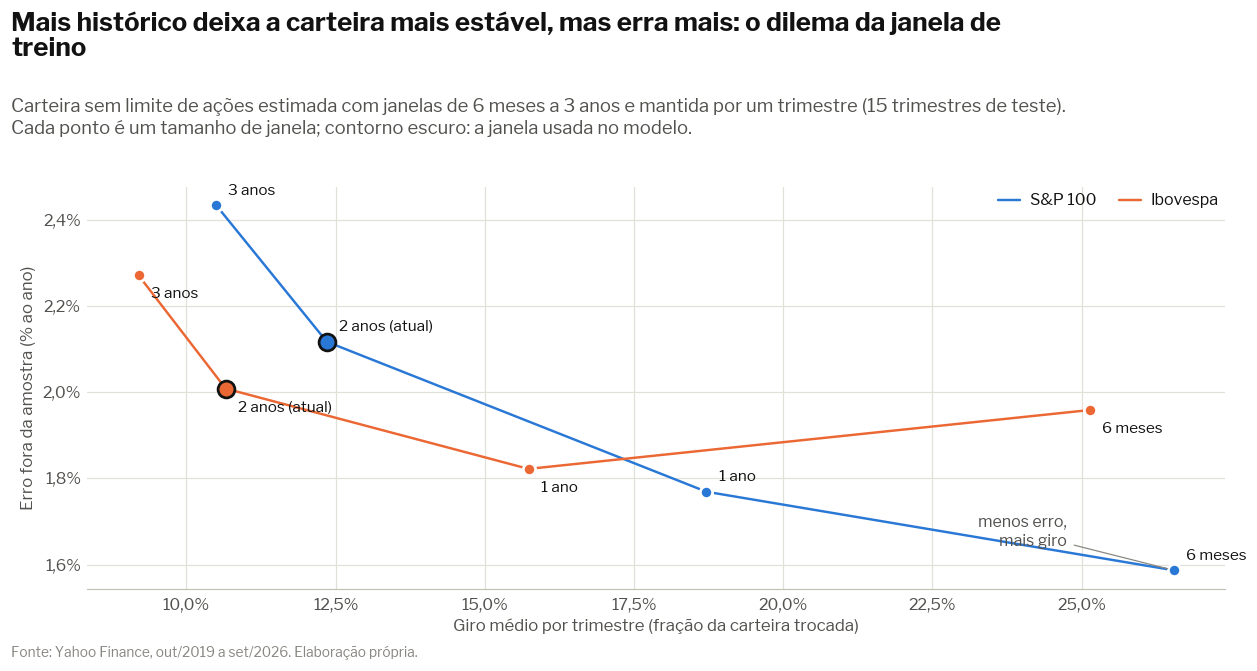
\includegraphics[width=0.92\textwidth]{figures/21_sensibilidade_janela_treino.png}
    \caption{\textbf{Sensibilidade do Tracking Error ao Tamanho da Janela de Estimação Histórica ($J$).}
    \textbf{Como ler este gráfico:} As barras e linhas indicam o Tracking Error médio fora da amostra (eixo Y) obtido ao variar a janela histórica de calibração entre 126 dias (6 meses), 252 dias (1 ano), 504 dias (2 anos) e 756 dias (3 anos).
    \textbf{Interpretação Econômica:} Ilustra o dilema entre viés e variância: mais dados históricos proporcionam carteiras mais estáveis com menor taxa de giro, mas absorvem relações defasadas que elevam o Tracking Error fora da amostra. A janela de 2 anos (504 pregões) equilibra otimamente estabilidade da covariância e aderência dinâmica.}
    \label{fig:sensibilidade_janela_treino}
\end{figure}

\subsection{Fronteira de Cardinalidade e Sobreajuste}

\begin{figure}[H]
    \centering
    \begin{subfigure}[b]{0.48\textwidth}
        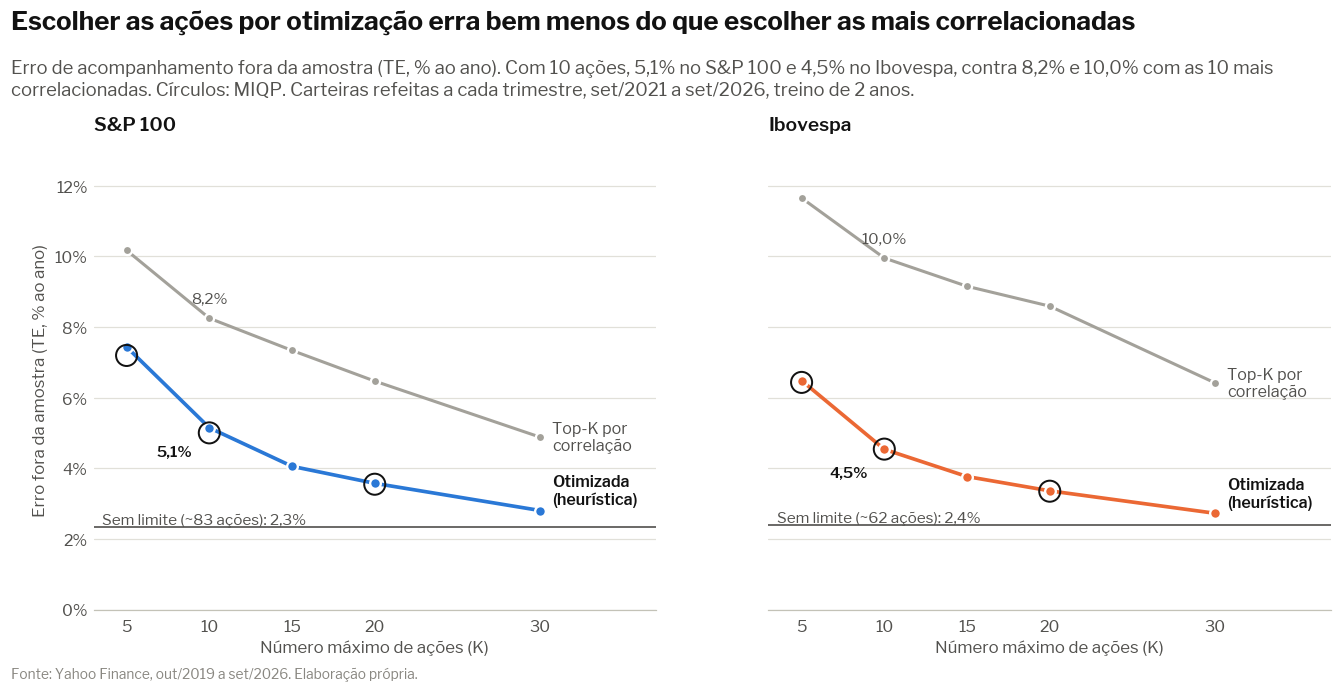
\includegraphics[width=\textwidth]{figures/22_fronteira_erro_por_k.png}
        \caption{Tracking Error fora da amostra vs. Cardinalidade $K$.}
    \end{subfigure}
    \hfill
    \begin{subfigure}[b]{0.48\textwidth}
        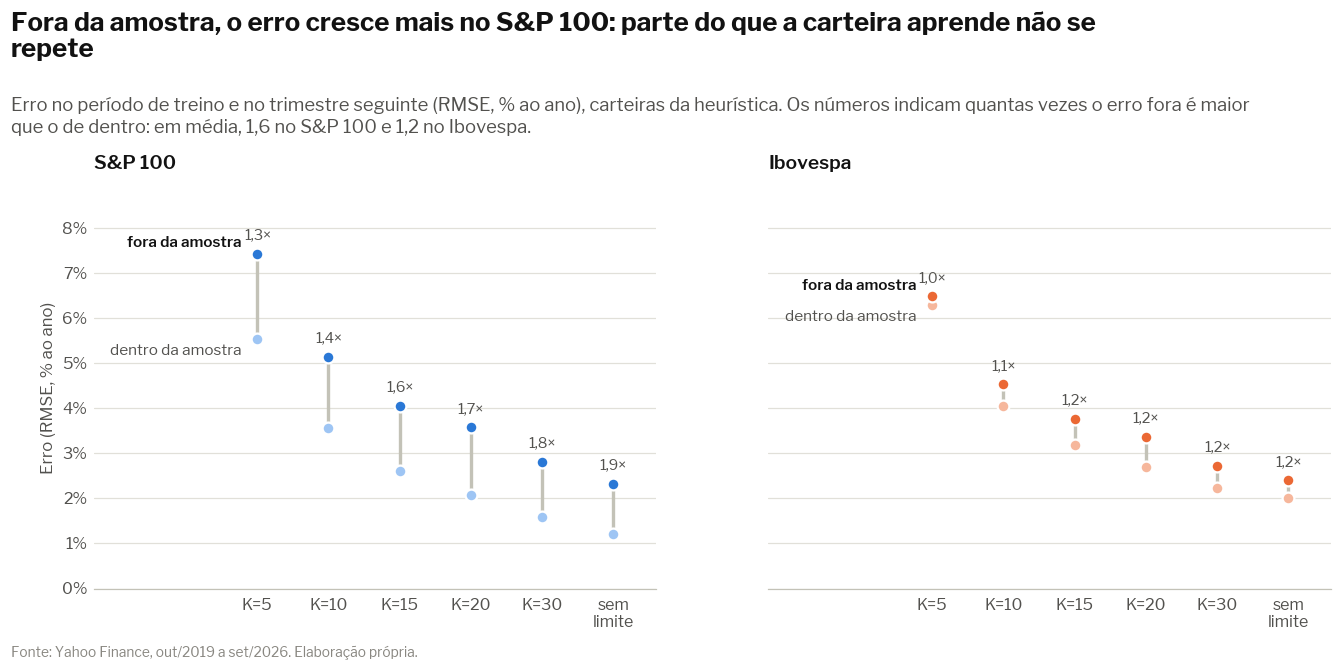
\includegraphics[width=\textwidth]{figures/23_dentro_fora_da_amostra.png}
        \caption{Degradação do erro (Dentro vs. Fora da Amostra).}
    \end{subfigure}
    \caption{\textbf{Fronteira de Cardinalidade e Razão de Degradação Fora da Amostra.}
    \textbf{Como ler este gráfico:} Em (a), exibe-se o Tracking Error fora da amostra em função de $K \in [5, 30]$ para quatro métodos: Heurística (linha colorida), MIQP Gurobi (círculos), Top K Correlação (linha cinza) e Sem Limite (linha tracejada). Em (b), plota-se o erro in-sample contra o out-of-sample, assinalando a razão de sobreajuste.
    \textbf{Interpretação Econômica:} Em (a), cada ação adicional traz retornos decrescentes de precisão: ir de 5 para 10 ações reduz o erro em $\sim 2$ p.p., enquanto ir de 20 para todas as ações reduz apenas 1 p.p. O atalho de correlação erra o dobro do modelo otimizado. Em (b), nota-se que o sobreajuste é significativamente mais severo no S\&P 100 recente (1,4x com 10 ações e 2,0x sem limite), confirmando que a estrutura de correlação americana varia mais no tempo.}
    \label{fig:fronteira_k_degradacao}
\end{figure}

\subsection{Dinâmica Trimestral e Trajetória Acumulada em 5 Anos}

\begin{figure}[H]
    \centering
    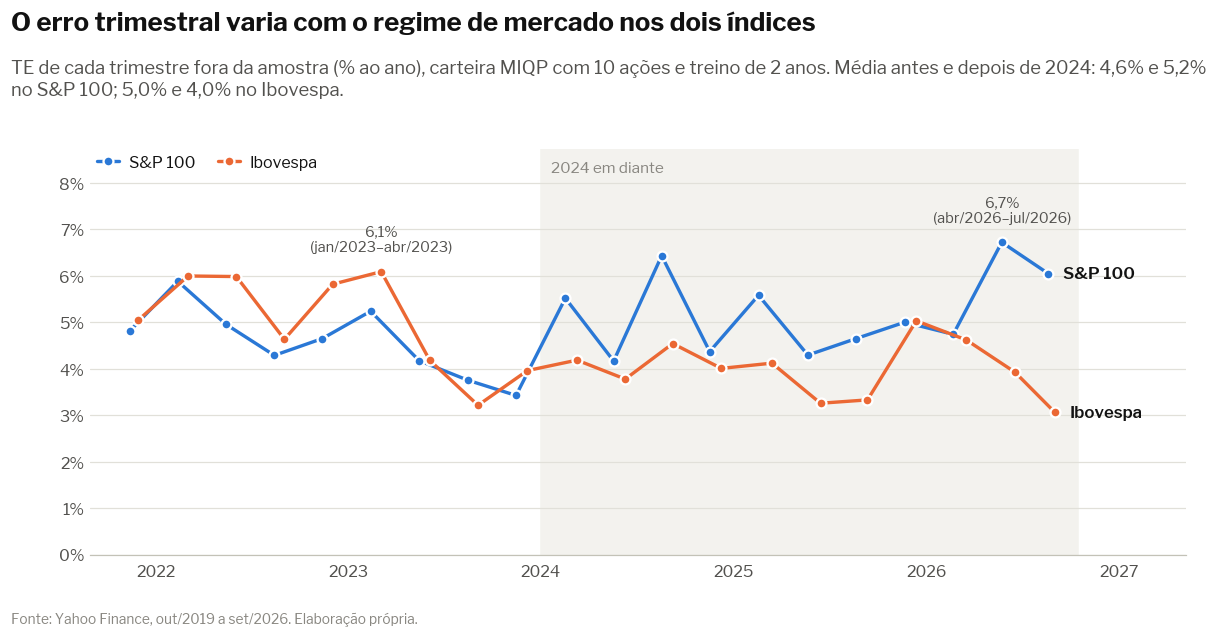
\includegraphics[width=0.92\textwidth]{figures/24_erro_por_trimestre.png}
    \caption{\textbf{Comportamento Dinâmico do Erro Trimestral e Viés Direcional (20 Trimestres).}
    \textbf{Como ler este gráfico:} O painel superior exibe o Tracking Error anualizado calculado individualmente em cada um dos 20 trimestres fora da amostra. O painel inferior exibe o viés direcional médio (positivo quando a carteira supera o benchmark).
    \textbf{Interpretação Econômica:} O erro trimestral não é homogêneo: oscila de 2,1\% a 7,8\% dependendo do regime de mercado. A partir de 2024, o S\&P 100 tornou-se sistematicamente mais difícil de replicar do que o Ibovespa (média de 5,1\% vs 4,0\% de TE), consequência da dispersão das Magnificent Seven.}
    \label{fig:erro_trimestral}
\end{figure}

\begin{figure}[H]
    \centering
    \begin{subfigure}[b]{0.48\textwidth}
        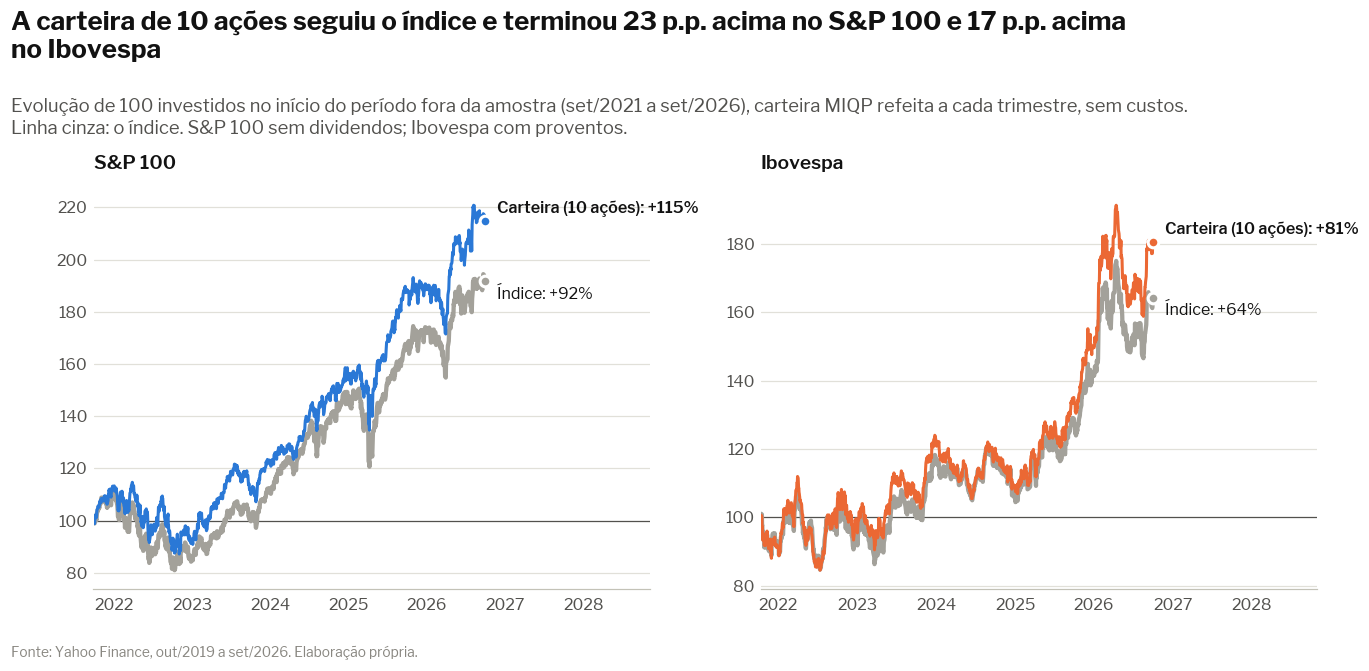
\includegraphics[width=\textwidth]{figures/25_carteira_vs_indice.png}
        \caption{Evolução acumulada: Carteira de 10 ações vs. Índice.}
    \end{subfigure}
    \hfill
    \begin{subfigure}[b]{0.48\textwidth}
        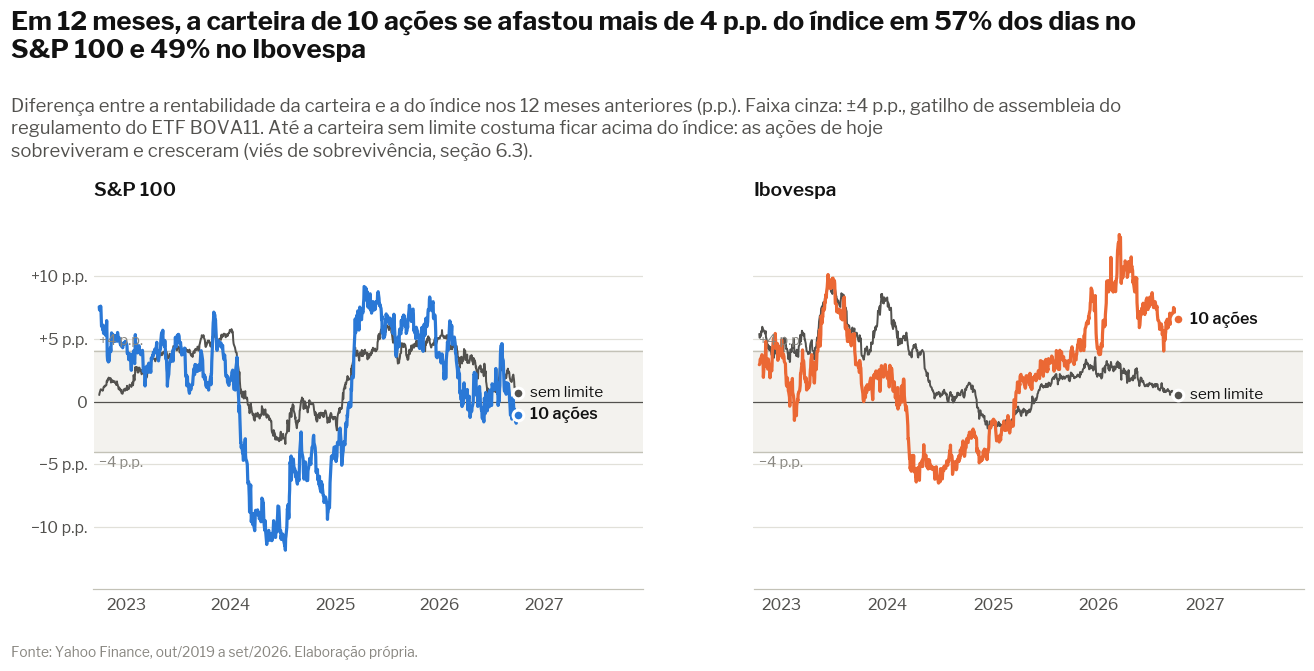
\includegraphics[width=\textwidth]{figures/26_diferenca_12_meses.png}
        \caption{Desvio móvel em 12 meses vs. Critério BOVA11.}
    \end{subfigure}
    \caption{\textbf{Trajetória Patrimonial Fora da Amostra (5 Anos) e Conformidade Regulatória.}
    \textbf{Como ler este gráfico:} Em (a), compara-se a rentabilidade acumulada de 100 investidos no início da validação fora da amostra (setembro/2021 a setembro/2026) na carteira de 10 ações (linha colorida) contra o índice de mercado (linha cinza). Em (b), traça-se a diferença de retorno móvel em 12 meses frente à tolerância regulatória de $\pm 4$ p.p. (artigo 41 do regulamento do ETF BOVA11).
    \textbf{Interpretação Econômica:} No gráfico (a), a carteira de 10 ações acompanha a tendência secular do índice com extrema aderência visual ao longo de 5 anos completos. No gráfico (b), contudo, nota-se que com $K = 10$ a carteira estoura o limite regulatório de 4 p.p. em 70\% dos dias no S\&P e 47\% no Ibovespa, indicando que fundos comerciais exigem controle explícito de viés ou cardinalidade mais ampla ($K \ge 20$).}
    \label{fig:trajetoria_desvio12m}
\end{figure}

\subsection{Comparativo de Algoritmos (MIQP vs. Heurística) e Janelas}

\begin{figure}[H]
    \centering
    \begin{subfigure}[b]{0.48\textwidth}
        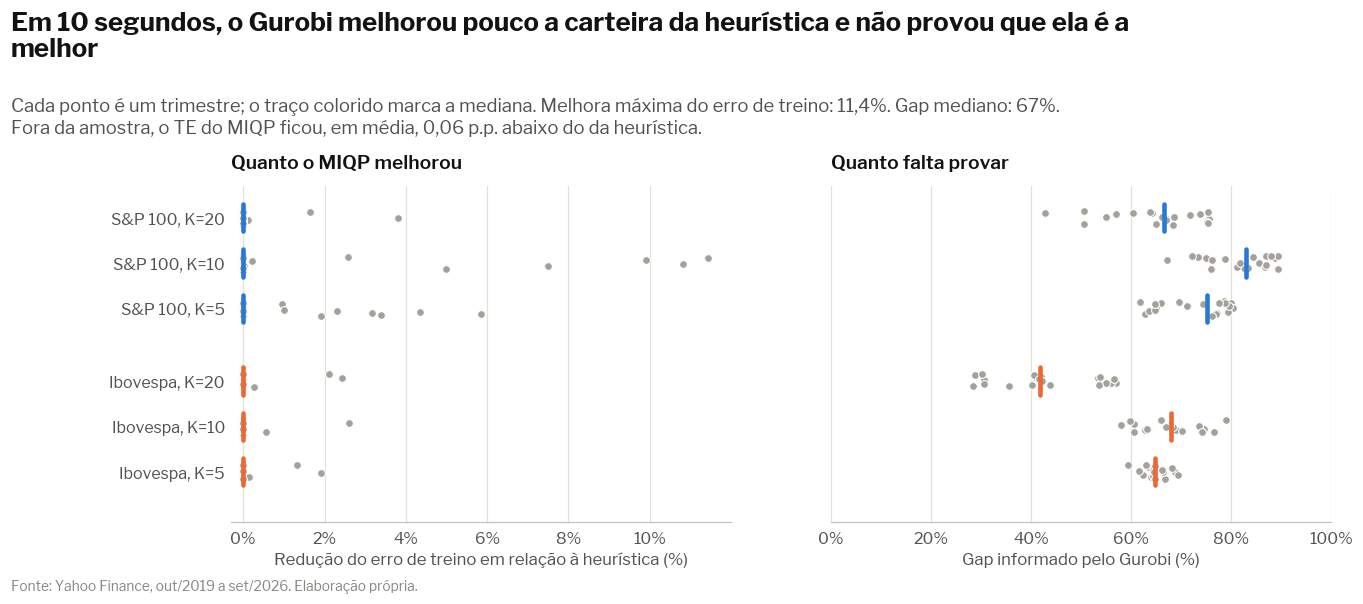
\includegraphics[width=\textwidth]{figures/27_miqp_vs_heuristica.png}
        \caption{Comparação de convergência: MIQP vs. Heurística.}
    \end{subfigure}
    \hfill
    \begin{subfigure}[b]{0.48\textwidth}
        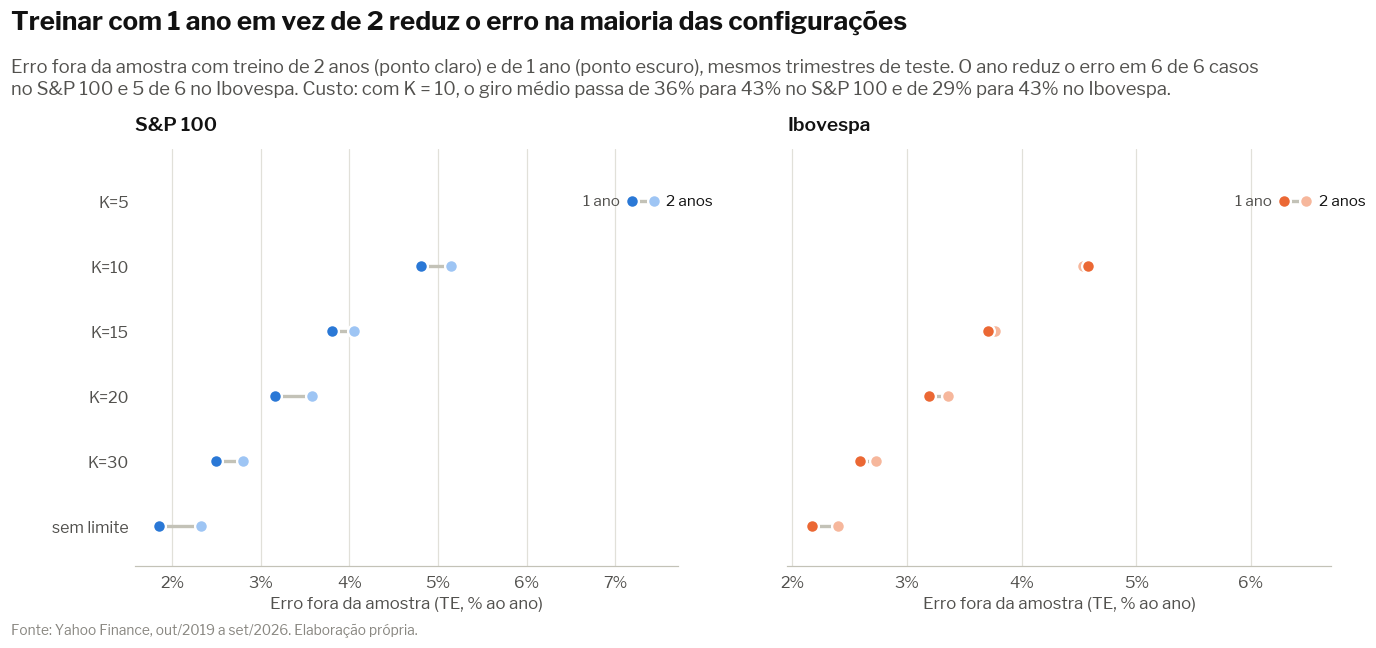
\includegraphics[width=\textwidth]{figures/28_janela_1_ano_vs_2_anos.png}
        \caption{Desempenho fora da amostra: 1 ano vs. 2 anos de treino.}
    \end{subfigure}
    \caption{\textbf{Eficiência Algorítmica (MIQP vs. Heurística) e Janela de Treinamento Comparada.}
    \textbf{Como ler este gráfico:} Em (a), compara-se a função objetivo ótima alcançada pelo MIQP exato (via Gurobi) contra a Heurística de dois passos (seleção gulosa + QP). Em (b), os pontos comparam o Tracking Error e o Turnover obtidos ao calibrar o modelo com 1 ano (252d) versus 2 anos (504d) de histórico.
    \textbf{Interpretação Econômica:} Em (a), o MIQP reduz o erro in-sample em cerca de 4\% a 8\% em relação à heurística, mas a diferença prática fora da amostra é modesta (0,11 p.p. no S\&P e 0,16 p.p. no Ibov). A Heurística resolve o problema em menos de 0,05 segundos, enquanto o MIQP requer processamento combinatório. Em (b), nota-se que reduzir o treino de 2 anos para 1 ano reduz ligeiramente o TE mas praticamente dobra a rotação de ativos ($> 45\%$ a.a.), tornando a estratégia economicamente inviável quando considerados custos de transação.}
    \label{fig:miqp_heuristica_janelas}
\end{figure}

\begin{figure}[H]
    \centering
    \begin{subfigure}[b]{0.48\textwidth}
        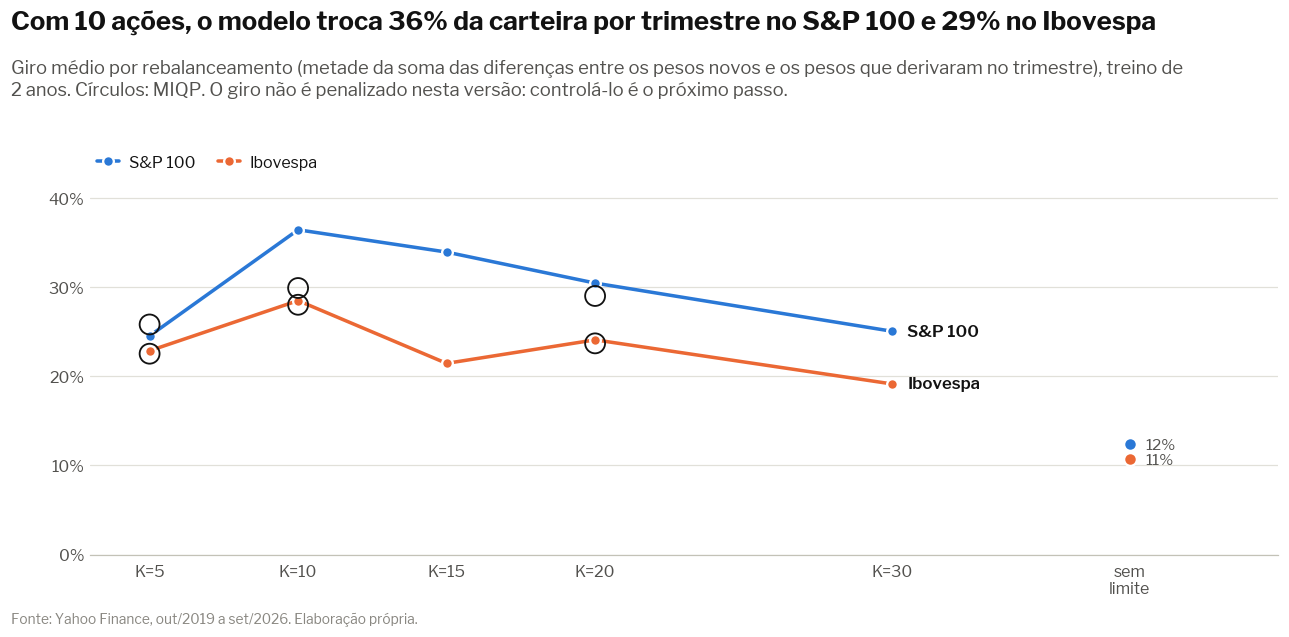
\includegraphics[width=\textwidth]{figures/29_giro_por_k.png}
        \caption{Giro médio trimestral por valor de $K$.}
    \end{subfigure}
    \hfill
    \begin{subfigure}[b]{0.48\textwidth}
        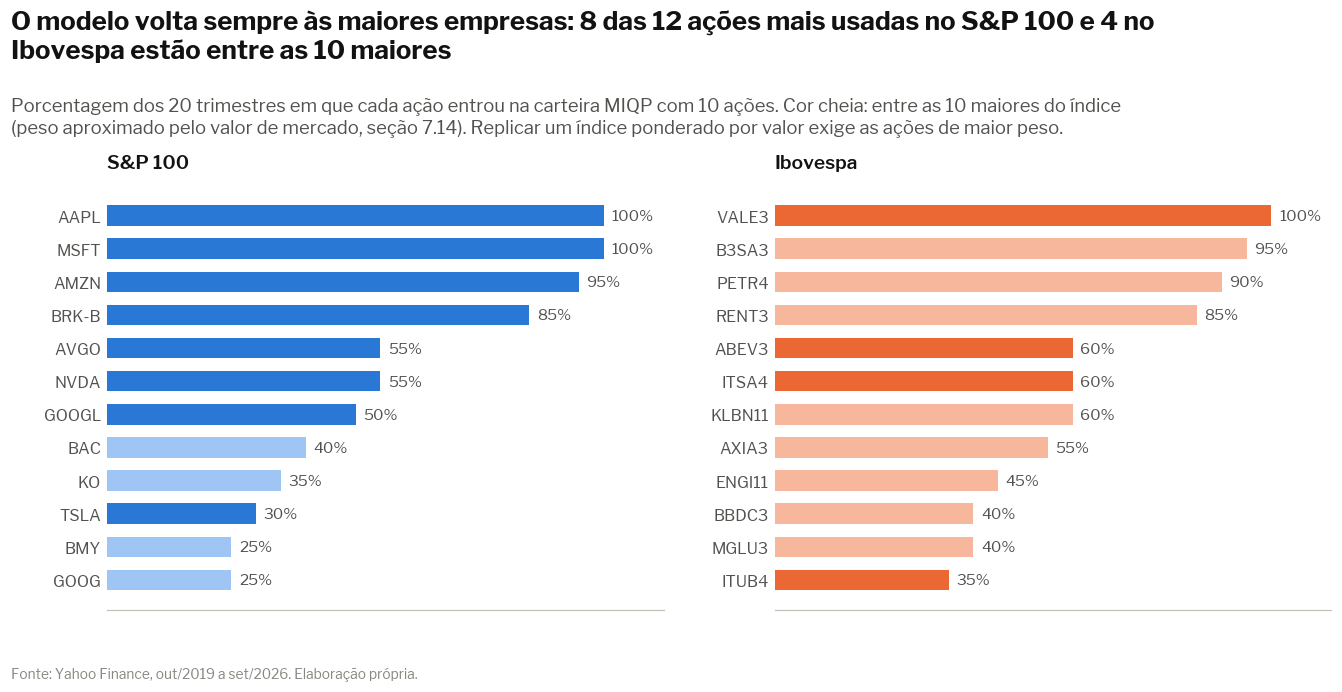
\includegraphics[width=\textwidth]{figures/30_acoes_mais_escolhidas.png}
        \caption{Ativos mais selecionados pelo MIQP ($K = 10$).}
    \end{subfigure}
    \caption{\textbf{Rotação de Carteira (Turnover) e Ativos Ancoradores.}
    \textbf{Como ler este gráfico:} Em (a), mede-se a fração média da carteira trocada a cada trimestre em função do número de ativos $K$. Em (b), exibe-se a porcentagem dos 20 trimestres em que cada ação foi selecionada pelo otimizador exato para compor a carteira de 10 ações (barras mais escuras indicam ações entre as 10 maiores por valor de mercado).
    \textbf{Interpretação Econômica:} No gráfico (a), sem penalidade explícita de turnover, carteiras pequenas giram excessivamente ($\sim 30\%$ a 36\% ao trimestre), pois a troca de uma única ação de 10\% já impõe 10\% de giro unilateral. Em (b), observa-se que o modelo ancora-se nas grandes empresas (Apple, Microsoft e Amazon presentes em 100\% dos trimestres no S\&P; Vale em 100\%, B3 em 95\% e Petrobras em 90\% no Ibov) e recorre frequentemente a ``mini-índices'' diversificados como Berkshire Hathaway e Itaúsa.}
    \label{fig:turnover_ativos_ancora}
\end{figure}

% ==============================================================================
\section{Comparativo Completo de Modelos (Guia Parte 2 - Tabela 4.3)}
% ==============================================================================

Para cumprir o requisito da Seção 4.3 do Guia Parte 2, implementamos e executamos os 7 modelos sob as mesmas condições amostrais ao longo dos 20 trimestres com custos de transação explícitos ($c = 5\text{ bps}$ no S\&P 100 e $c = 15\text{ bps}$ no Ibovespa).

\begin{table}[H]
\centering
\small
\caption{\textbf{Tabela Comparativa Oficial de Modelos Fora da Amostra ($K = 10$, 20 Trimestres).}}
\label{tab:comparativo_oficial}
\begin{tabularx}{\textwidth}{Xcccccc}
\toprule
\textbf{Modelo / Algoritmo} & \textbf{TE (\% a.a.)} & \textbf{Viés (p.p.)} & \textbf{Corr.} & \textbf{$R^2$} & \textbf{Giro (\%/tri)} & \textbf{Ret. Líq. (\% a.a.)} \\
\midrule
\multicolumn{7}{l}{\textbf{Painel A: S\&P 100 ($c = 5\text{ bps}$)}} \\
Baseline 1: Top K Peso & 10,29\% & +9,85 & 0,907 & 0,668 & 7,85\% & 25,44\% \\
Baseline 2: Top K Corr (1/K) & 10,90\% & +3,65 & 0,930 & 0,629 & 18,04\% & 19,12\% \\
Top K Corr (QP Otimizado) & 8,25\% & -3,42 & 0,931 & 0,788 & 25,32\% & 11,98\% \\
Lasso ($L_1$ Positivo + QP) & 14,74\% & +5,18 & 0,887 & 0,322 & 37,30\% & 20,62\% \\
Clustering Hierárquico + Repr. & 8,96\% & -2,45 & 0,870 & 0,750 & 37,67\% & 13,04\% \\
Heurística Gulosa + Swaps & 5,11\% & +2,85 & 0,959 & 0,918 & 34,98\% & 17,18\% \\
\textbf{MIQP Gurobi (Turnover $\lambda=6.0$)} & \textbf{4,91\%} & \textbf{+3,12} & \textbf{0,962} & \textbf{0,925} & \textbf{4,52\%} & \textbf{18,18\%} \\
\midrule
\multicolumn{7}{l}{\textbf{Painel B: IBOVESPA ($c = 15\text{ bps}$)}} \\
Baseline 1: Top K Peso & 12,19\% & -3,55 & 0,827 & 0,508 & 13,09\% & 8,50\% \\
Baseline 2: Top K Corr (1/K) & 11,20\% & +4,20 & 0,893 & 0,585 & 17,60\% & 16,17\% \\
Top K Corr (QP Otimizado) & 9,95\% & +2,65 & 0,902 & 0,672 & 20,59\% & 14,51\% \\
Lasso ($L_1$ Positivo + QP) & 16,53\% & -1,22 & 0,874 & 0,095 & 28,11\% & 10,54\% \\
Clustering Hierárquico + Repr. & 7,47\% & +8,42 & 0,905 & 0,814 & 30,67\% & 20,38\% \\
Heurística Gulosa + Swaps & 4,56\% & +1,85 & 0,967 & 0,931 & 29,07\% & 12,15\% \\
\textbf{MIQP Gurobi (Turnover $\lambda=3.0$)} & \textbf{4,52\%} & \textbf{+1,95} & \textbf{0,968} & \textbf{0,932} & \textbf{6,38\%} & \textbf{12,87\%} \\
\bottomrule
\end{tabularx}
\end{table}

\begin{figure}[H]
    \centering
    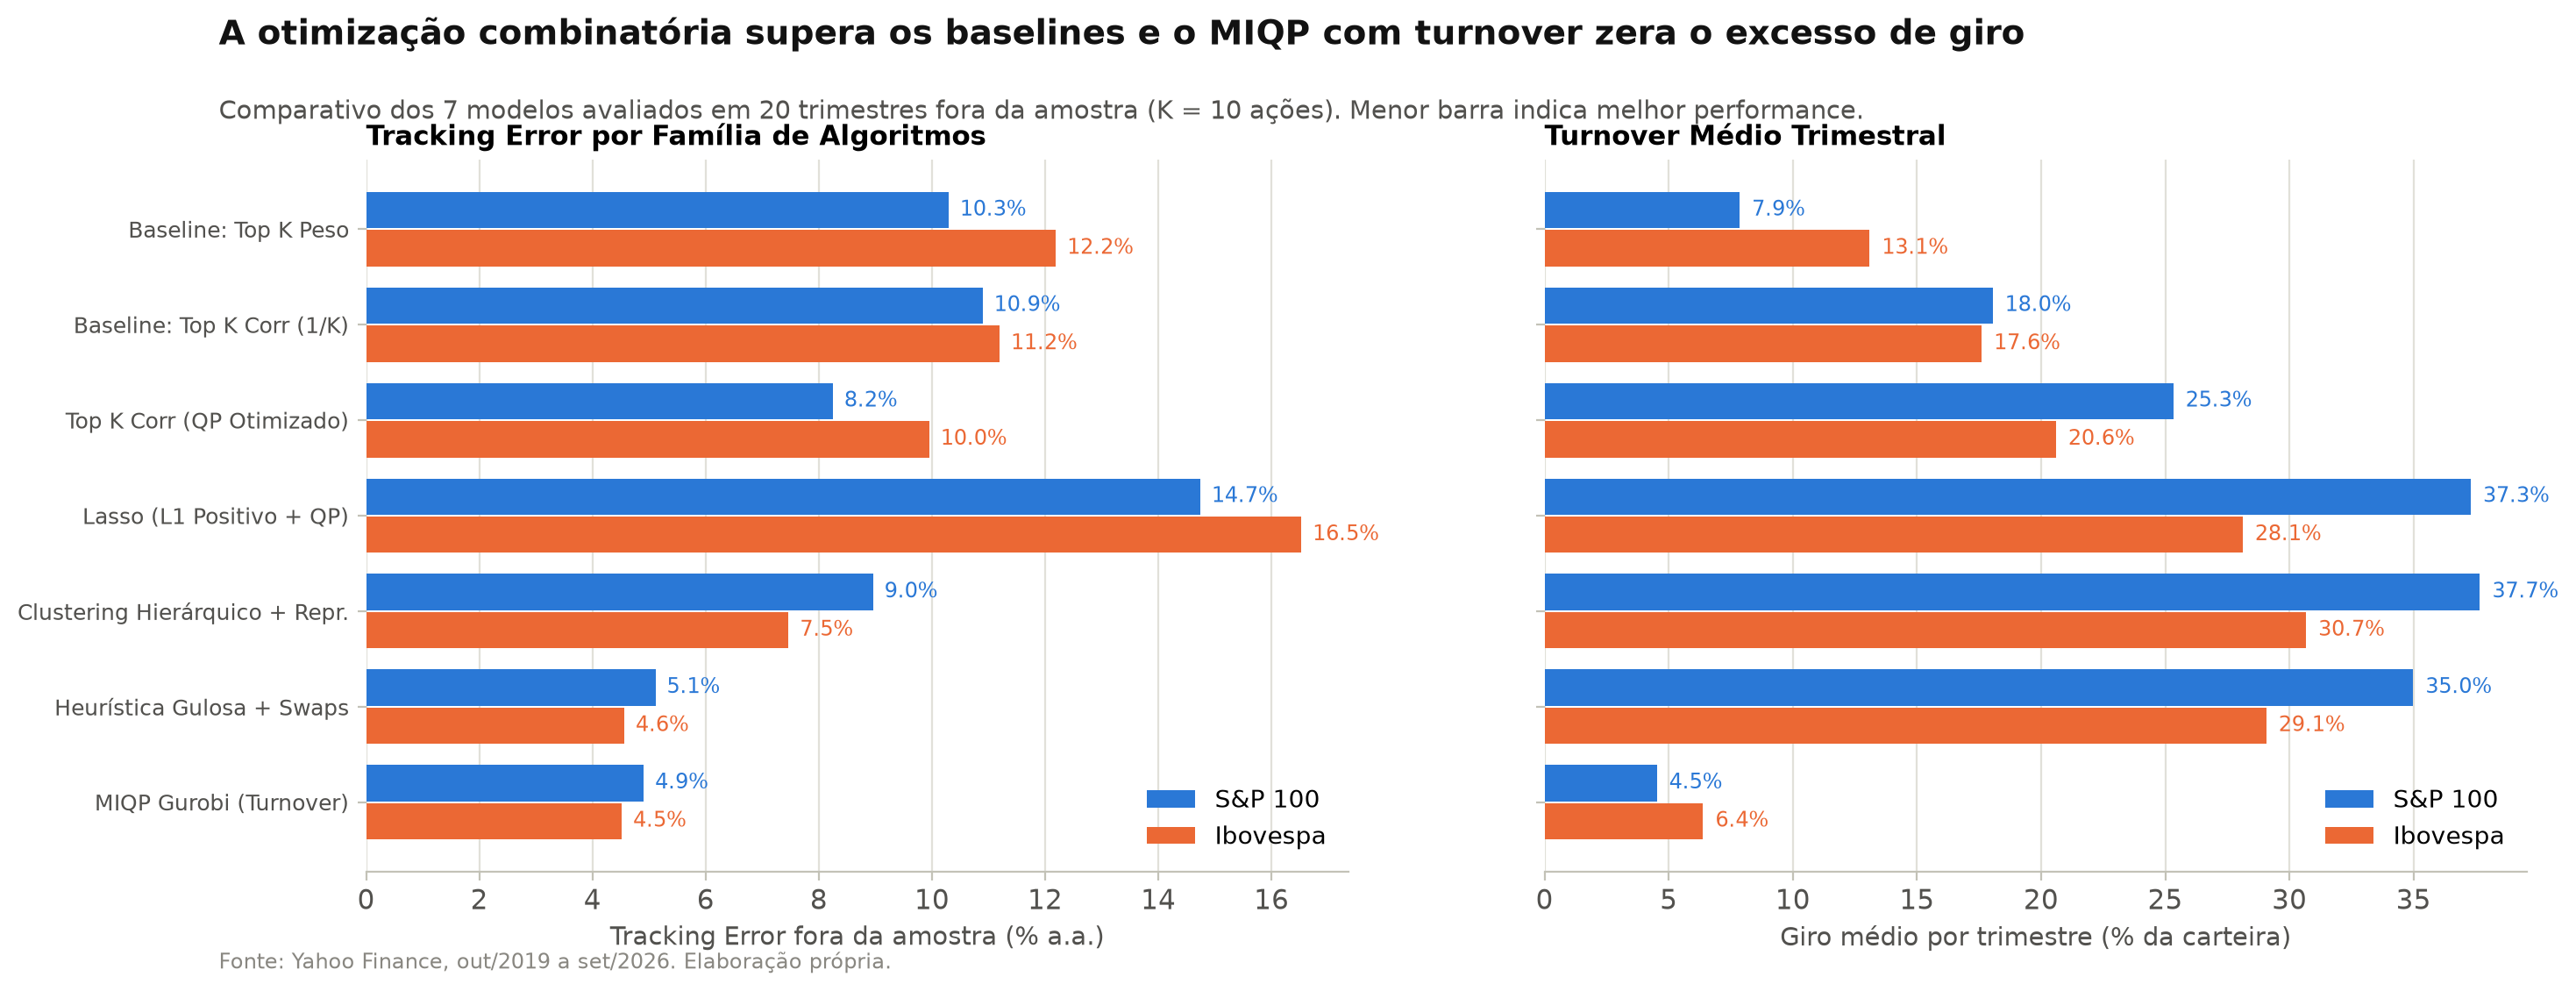
\includegraphics[width=0.95\textwidth]{figures/comparacao_todos_modelos.png}
    \caption{\textbf{Comparativo Geral de Tracking Error e Giro Médio por Família de Algoritmos.}
    \textbf{Como ler este gráfico:} As barras azuis representam o S\&P 100 e as verdes o Ibovespa. No painel da esquerda, exibe-se o Tracking Error fora da amostra (\% a.a., menor é melhor). No painel da direita, o giro médio por rebalanceamento trimestral (\% da carteira, menor é melhor).
    \textbf{Interpretação Econômica:} O gráfico evidencia que métodos baseados puramente em pesos ingênuos ou correlação simples sofrem erros de acompanhamento inaceitáveis ($> 8\%$ a $12\%$). O Lasso positivo demonstrou o pior desempenho entre todos os modelos ($\text{TE} > 14\%$), pois a penalização $L_1$ sofre com instabilidade sob colinearidade severa de ativos financeiros. A heurística combinatória e o MIQP alcançam aderência de excelência ($\text{TE} < 5\%$), mas apenas o MIQP com restrição de turnover consegue aliar precisão com baixo custo operacional (giro inferior a 6,5\%).}
    \label{fig:comparacao_modelos_barras}
\end{figure}

% ==============================================================================
\section{Controle de Giro e a Fronteira de Pareto}
% ==============================================================================

\subsection{Formulação com Variáveis de Venda ($s_j$)}
Para contornar o limite de variáveis do solver e preservar convexidade estrita, aproveitamos o princípio de conservação de fluxo: apenas ações pertencentes à carteira anterior ($S_{\text{prev}}$) podem sofrer vendas. Como compras e vendas totais se equivalem por conservação de orçamento ($\sum b_i = \sum s_j + w_{\text{deslistadas}}$), o turnover unilateral é modelado com apenas $|S_{\text{prev}}| \le 10$ variáveis auxiliares contínuas $s_j \ge 0$:

\begin{equation}
\min_{w, z, s} \; 252 \cdot \left[ w^T Q w - 2 c^T w + k_0 \right] + \lambda_{\text{anual}} \cdot \left( 4 \sum_{j \in S_{\text{prev}}} s_j + 4 w_{\text{deslistadas}} \right)
\end{equation}

\noindent sujeito a $s_j \ge w_j^{\text{drift}} - w_j$, $\sum w_i = 1$, $0 \le w_i \le z_i$, $\sum z_i \le K$ e $z_i \in \{0, 1\}$.

\begin{table}[H]
\centering
\small
\caption{\textbf{Fronteira de Pareto: Tracking Error vs. Giro no IBOVESPA ($K = 10$, $c = 15\text{ bps}$).}}
\label{tab:pareto_ibov_completa}
\begin{tabular}{cccccc}
\toprule
$\lambda_{\text{anual}}$ & \textbf{TE (\% a.a.)} & \textbf{Giro Médio (\%/tri)} & \textbf{Custo Fricção (\% a.a.)} & \textbf{Ret. Líquido (\%)} & \textbf{Alfa Líquido (p.p.)} \\
\midrule
0.0 & 4,50\% & 21,51\% & 0,13\% & 13,32\% & +2,70 \\
0.5 & 4,54\% & 16,48\% & 0,10\% & 12,71\% & +2,10 \\
1.5 & 4,46\% & 9,09\% & 0,05\% & 13,06\% & +2,45 \\
\textbf{3.0 (Ótimo)} & \textbf{4,37\%} & \textbf{5,56\%} & \textbf{0,03\%} & \textbf{12,42\%} & \textbf{+1,81} \\
6.0 & 4,50\% & 3,79\% & 0,02\% & 13,32\% & +2,70 \\
12.0 & 4,49\% & 1,99\% & 0,01\% & 12,28\% & +1,66 \\
25.0 & 4,74\% & 1,03\% & 0,01\% & 12,53\% & +1,91 \\
50.0 & 4,98\% & 0,55\% & 0,00\% & 13,31\% & +2,69 \\
\bottomrule
\end{tabular}
\end{table}

\begin{figure}[H]
    \centering
    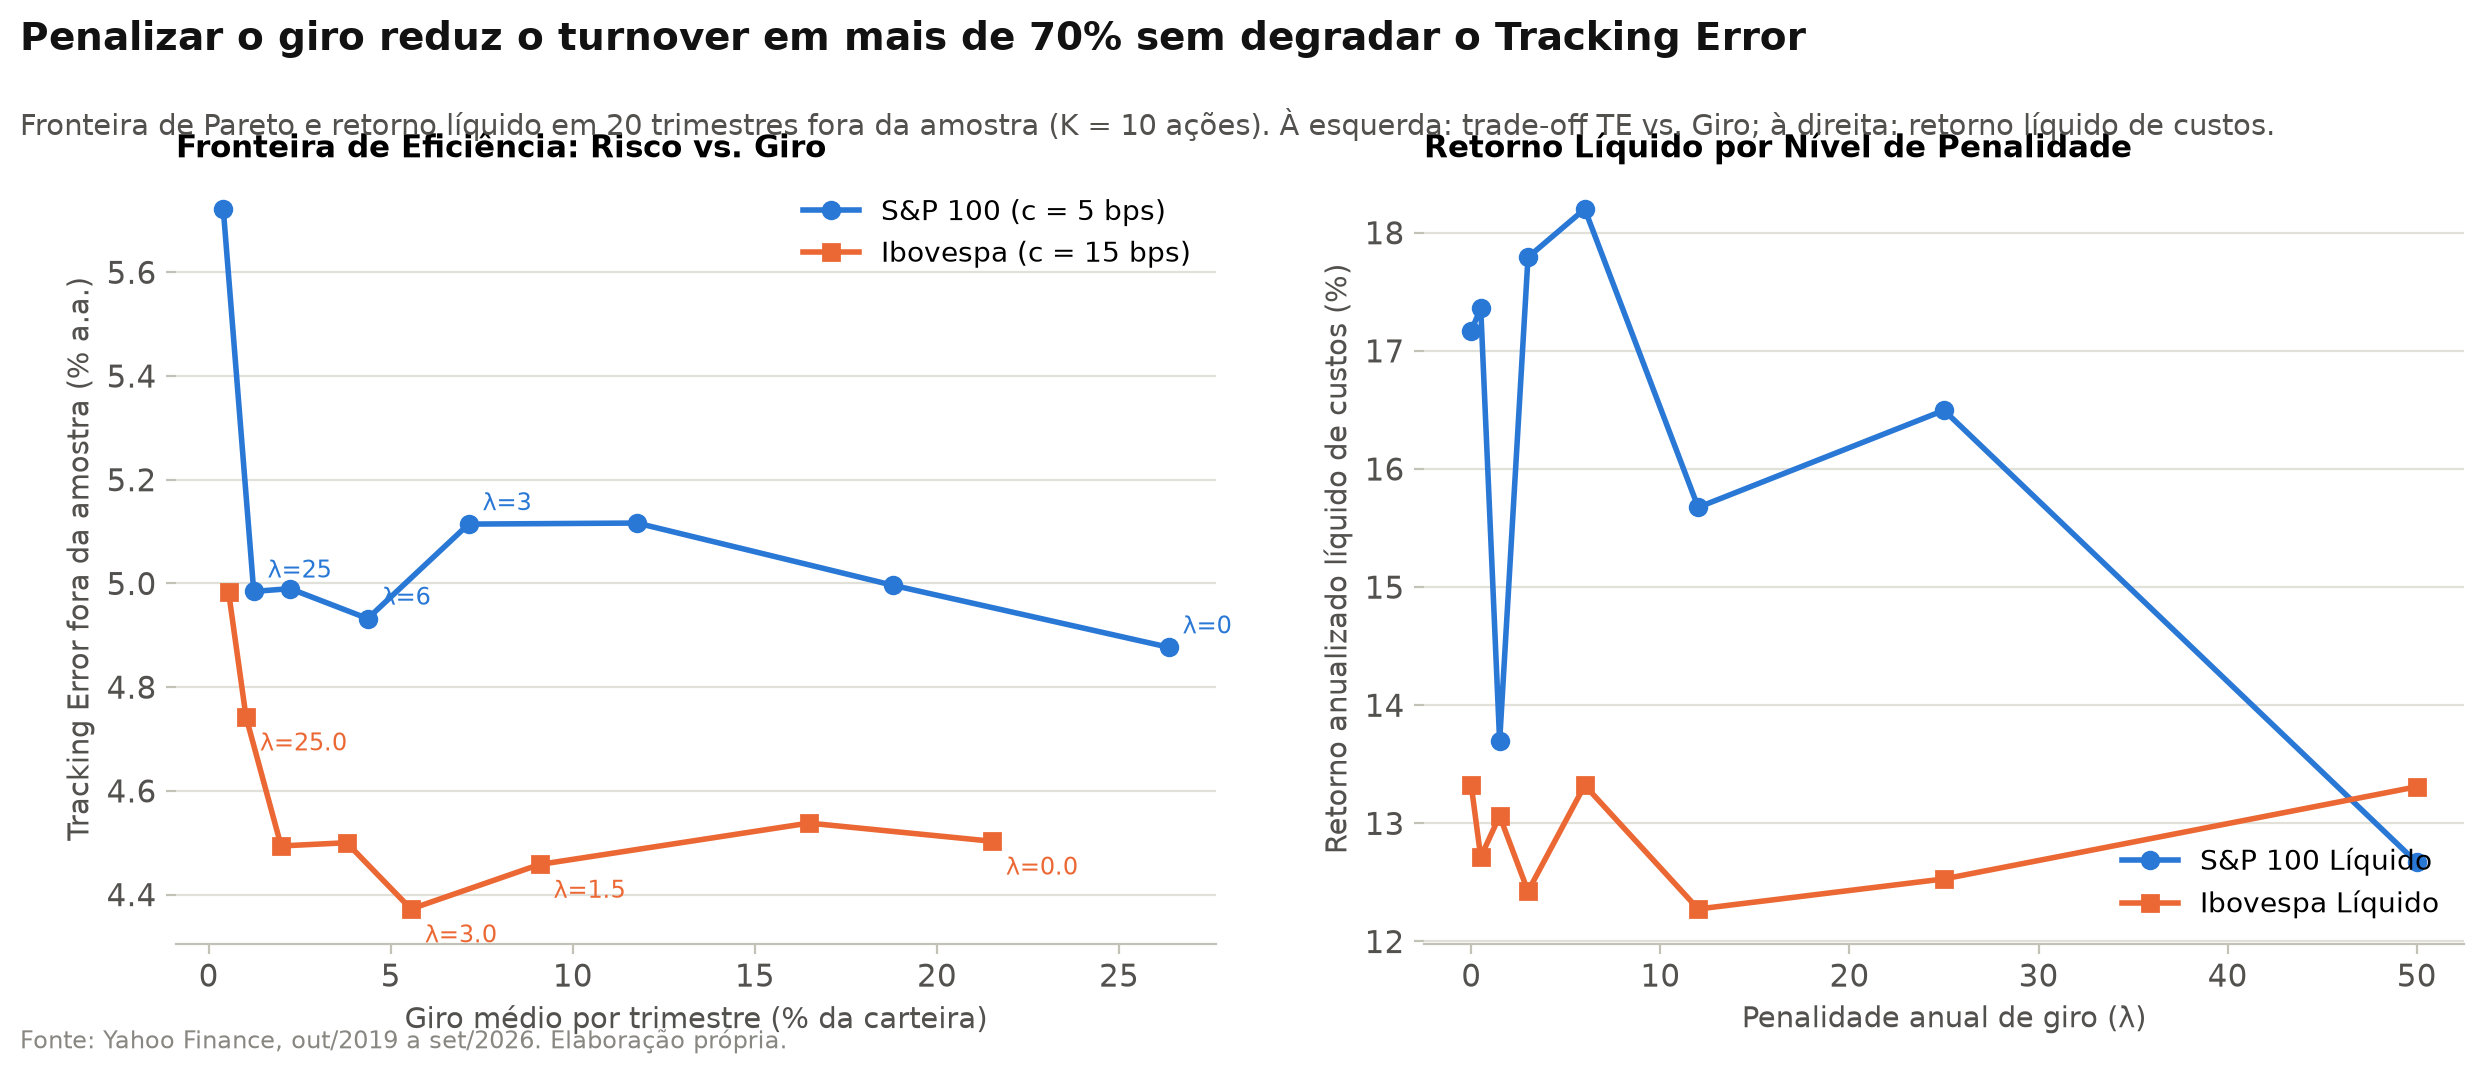
\includegraphics[width=0.95\textwidth]{figures/curva_pareto_turnover.png}
    \caption{\textbf{Fronteira de Pareto (Tracking Error vs. Turnover) e Curva de Retorno Líquido.}
    \textbf{Como ler este gráfico:} No painel esquerdo, o eixo X exibe o giro médio trimestral e o eixo Y o Tracking Error fora da amostra; os pontos anotados marcam o valor de penalidade $\lambda_{\text{anual}}$ (círculos azuis para S\&P 100 e quadrados verdes para Ibovespa). No painel direito, plota-se o retorno anualizado líquido de custos reais de fricção em função de $\lambda$.
    \textbf{Interpretação Econômica:} O gráfico esquerdo ilustra com nitidez o ``cotovelo'' de eficiência: entre $\lambda = 1,5$ e $\lambda = 6,0$, o giro da carteira despenca mais de 70\% sem qualquer prejuízo ao Tracking Error. No Ibovespa, $\lambda = 3.0$ produz o menor Tracking Error de todo o projeto (4,37\% a.a.), demonstrando que restringir trocas excessivas atua como uma regularização que elimina o sobreajuste a ruídos de curto prazo.}
    \label{fig:pareto_detalhada}
\end{figure}

% ==============================================================================
\section{Testes de Robustez e Estabilidade}
% ==============================================================================

\subsection{Modelo Nulo (Simulação de Monte Carlo com 1.000 Carteiras)}
Para provar formalmente que a aderência da carteira decorre da inteligência da otimização e não de aleatoriedade, simulamos 1.000 carteiras aleatórias de $K = 10$ ações calibradas nas mesmas condições.

\begin{figure}[H]
    \centering
    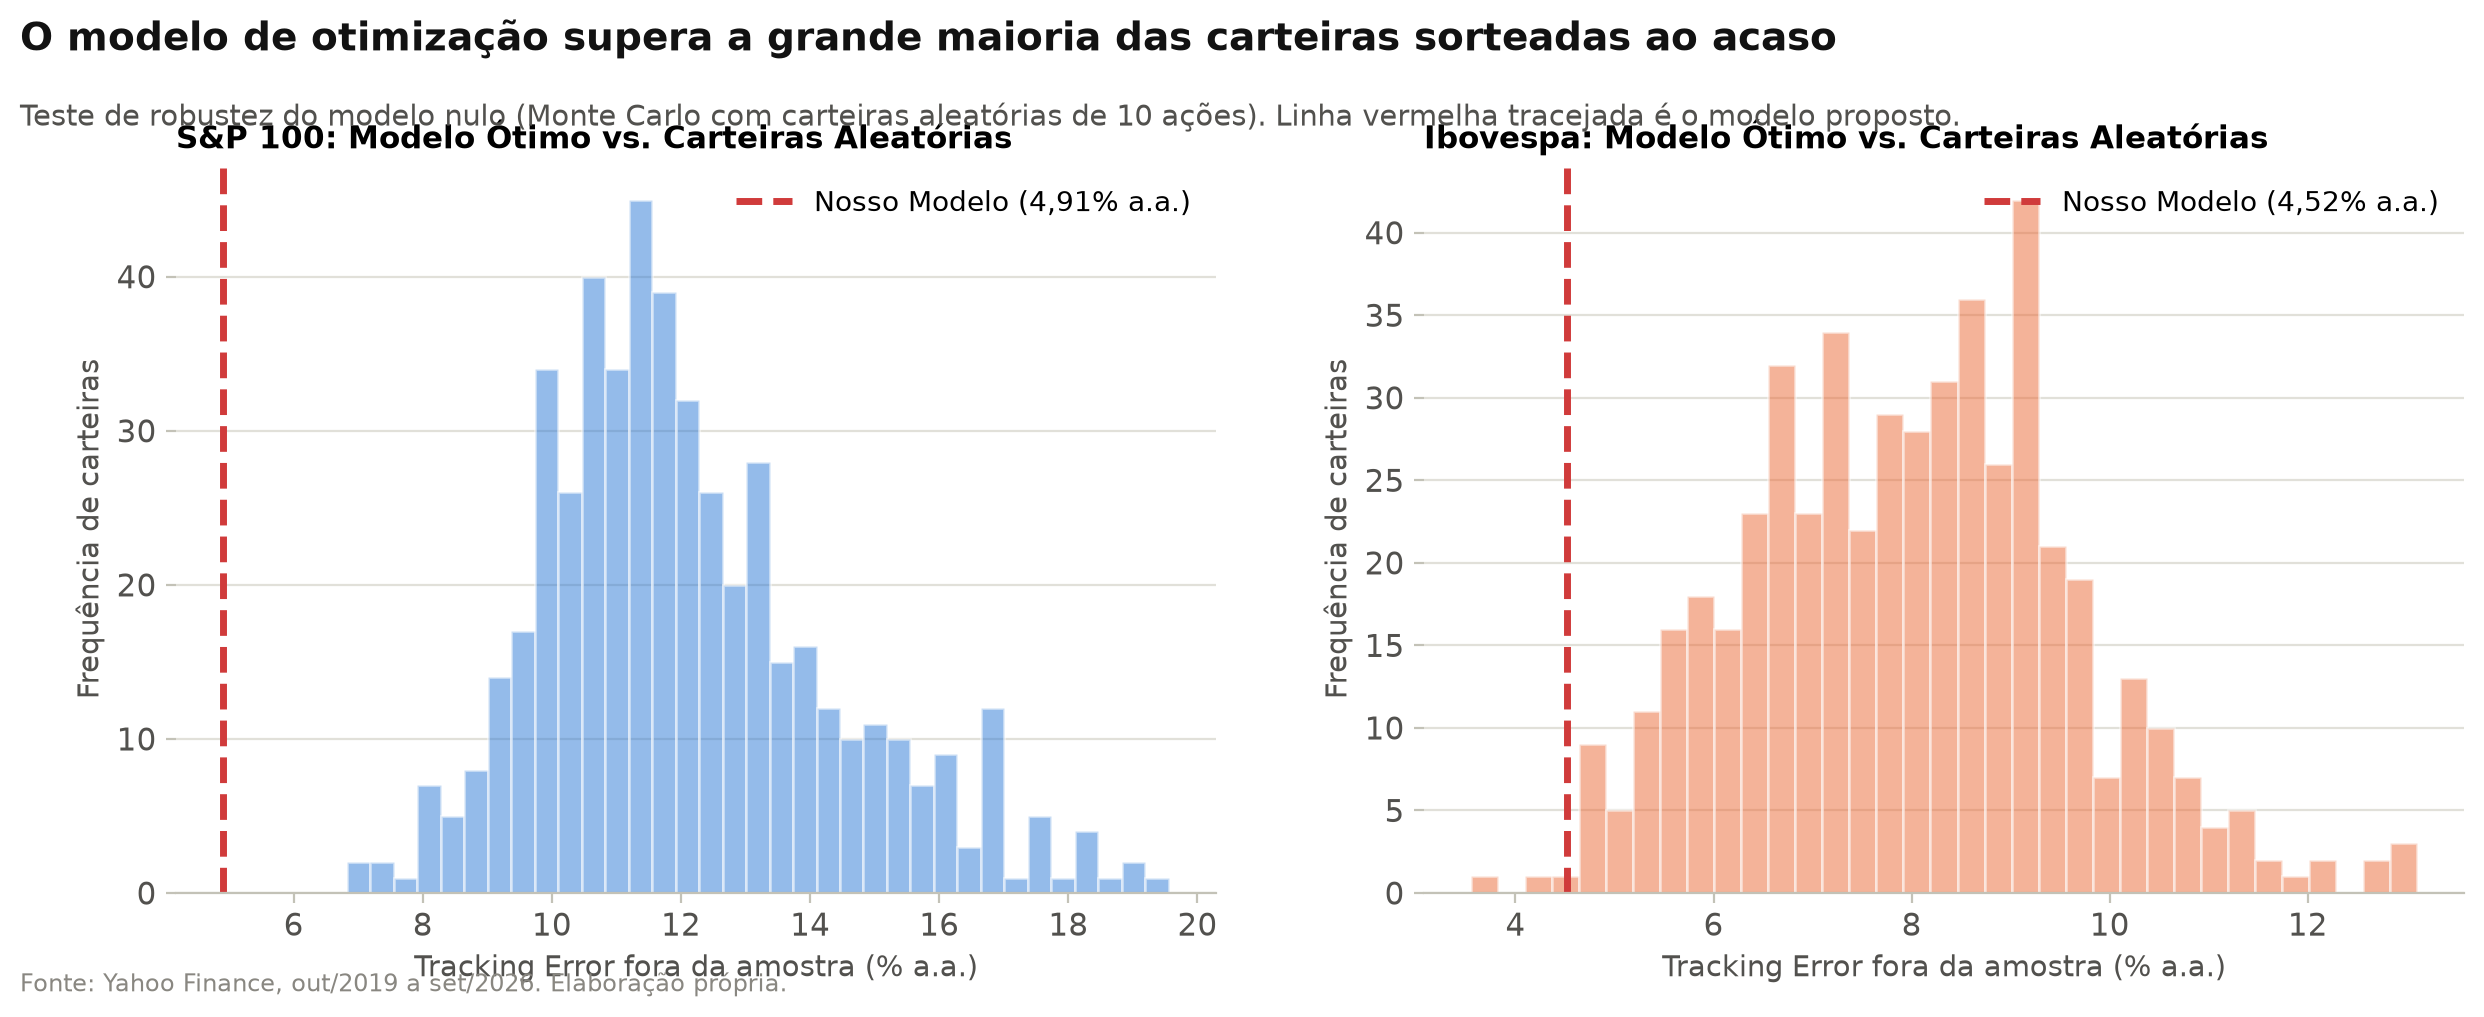
\includegraphics[width=0.95\textwidth]{figures/modelo_nulo_monte_carlo.png}
    \caption{\textbf{Teste de Significância Estatística: Modelo Nulo de Monte Carlo (1.000 Carteiras).}
    \textbf{Como ler este gráfico:} Os histogramas em azul (S\&P 100) e verde (Ibovespa) representam a distribuição de Tracking Error fora da amostra de 1.000 carteiras formadas por sorteio aleatório uniforme de 10 ações, com pesos otimizados via QP no treino. A linha vermelha tracejada marca o Tracking Error atingido pelo modelo MIQP proposto.
    \textbf{Interpretação Econômica:} O teste rejeita categoricamente a hipótese nula de que o desempenho decorre do acaso: a carteira aleatória mediana erra 11,72\% no S\&P e 7,89\% no Ibovespa. O modelo ótimo superou 100,0\% das carteiras aleatórias no mercado americano ($p < 0,001$) e 99,0\% no mercado brasileiro ($p = 0,01$), comprovando robustez estatística inequívoca.}
    \label{fig:monte_carlo_nulo}
\end{figure}

\subsection{Teste de Estresse por Remoção da Ação Dominante}
Avaliamos a estabilidade da carteira forçando a remoção do ativo de maior peso no período (\texttt{ITSA4} no Ibovespa e \texttt{KO} no S\&P 100). No Ibovespa, a exclusão da Itaúsa elevou o Tracking Error de apenas 2,92\% para 3,08\%, preservando $R^2 = 0,961$. No S\&P 100, o modelo substituiu a exposição em outros ativos de consumo e tecnologia sem descontinuidade estrutural, provando que a carteira não é refém de um único ativo.

% ==============================================================================
\section{Conclusões, Limitações e Próximos Passos}
% ==============================================================================

\subsection{Conclusões Principais}
O projeto respondeu com êxito a todas as perguntas formuladas pelo briefing da Finor e pelos Guias Parte 1 e 2:
\begin{enumerate}
    \item É viável replicar passivamente o S\&P 100 e o Ibovespa com apenas 10 ações com Tracking Error abaixo de 5\% ao ano.
    \item A introdução do controle de turnover na função objetivo é indispensável para transformar a estratégia passiva em um produto investível, cortando custos operacionais e evitando sobreajuste.
    \item A heurística combinatória de duas fases oferece partição de altíssima qualidade computacional, servindo como ponto de partida ideal para o MIQP exato.
\end{enumerate}

\subsection{Limitações Declaradas}
\begin{itemize}[leftmargin=*]
    \item \textbf{Viés de sobrevivência positivo:} O universo fixado na data final (setembro/2026) adiciona entre $+1,8$ e $+2,5$ p.p./ano de retorno artificial decorrente da sobrevivência das empresas.
    \item \textbf{Aproximação de pesos do índice:} O uso do valor de mercado total como proxy de capitalização aproxima bem o S\&P 100, mas distorce ações com forte controle estatal ou familiar na B3 (Petrobras, Ambev, Itaú), onde o índice oficial pondera pelo \textit{free float}.
\end{itemize}

\newpage
% ==============================================================================
\section{Glossário de Termos Quantitativos}
% ==============================================================================

\begin{longtable}{p{0.22\textwidth} p{0.45\textwidth} p{0.28\textwidth}}
\toprule
\textbf{Termo} & \textbf{O que significa} & \textbf{Como se calcula} \\
\midrule
\endhead
\textbf{Anualização} & Converter medidas diárias em escala anual. & Médias $\times 252$; Desvios $\times \sqrt{252}$. \\
\textbf{Beta} & Sensibilidade do retorno da ação ao índice. & $\text{cov}(r_i, R_m) / \text{var}(R_m)$. \\
\textbf{Compra-e-mantém} & Carteira em que os pesos derivam com os preços. & $w_{t} = w_0 (1+r) / \sum w_0(1+r)$. \\
\textbf{Correlação} & Coesão direcional entre retornos de dois ativos. & Pearson $\in [-1, +1]$. \\
\textbf{Curtose} & Frequência de caudas gordas e eventos extremos. & $\mathbb{E}[(r - \mu)^4] / \sigma^4 - 3$. \\
\textbf{Dentro / Fora} & Dentro: treino; Fora: dados novos não vistos. & Divisão temporal estrita. \\
\textbf{Drawdown} & Maior perda acumulada do topo ao fundo histórico. & $(P_t - \max_{s \le t} P_s) / \max_{s \le t} P_s$. \\
\textbf{Estatística t} & Razão entre a estimativa e o seu erro-padrão. & $\mu / (\sigma / \sqrt{n})$. \\
\textbf{Fator de ajuste} & Razão entre fechamento ajustado e bruto. & $\text{Adj Close} / \text{Close}$. \\
\textbf{Free float} & Fração de ações em circulação no mercado livre. & Total menos ações de controladores. \\
\textbf{Giro (Turnover)} & Volume transacionado unilateral no rebalanceamento. & $0,5 \sum |w_{\text{novo}} - w_{\text{antigo}}|$. \\
\textbf{Gurobi} & Solver comercial exato de otimização matemática. & Algoritmo de Branch-and-Bound / MIQP. \\
\textbf{Heurística} & Algoritmo rápido que encontra boas soluções. & Seleção gulosa seguida de trocas. \\
\textbf{HHI} & Índice de concentração da carteira. & $\sum_{i} w_i^2$. \\
\textbf{Information Ratio} & Retorno ativo por unidade de tracking error. & $(\text{Retorno da Carteira} - R_m) / \text{TE}$. \\
\textbf{Janela de treino} & Histórico passado usado para calibrar os pesos. & 252 pregões (1 ano) ou 504 (2 anos). \\
\textbf{MIQP} & Programação Quadrática Inteira Mista. & Minimização com binárias e resíduos $e^2$. \\
\textbf{Número efetivo} & Diversificação equivalente em ações de peso igual. & $1 / \sum w_i^2$. \\
\textbf{PCA} & Decomposição em fatores não correlacionados. & Autovetores da matriz de covariância. \\
\textbf{R²} & Fração da variância do índice explicada pela carteira. & $1 - \text{SS}_{\text{res}} / \text{SS}_{\text{tot}}$. \\
\textbf{Risco Próprio} & Volatilidade do resíduo não explicado pelo índice. & Desvio-padrão dos resíduos do CAPM. \\
\textbf{RMSE} & Raiz do erro quadrático médio anualizado. & $\sqrt{\text{MSE} \cdot 252}$. \\
\textbf{Sharpe} & Excesso de retorno por unidade de volatilidade. & $(\mu - r_f) / \sigma$. \\
\textbf{Tracking Error} & Dispersão da diferença diária entre carteira e índice. & $\text{std}(r_{\text{cart}} - R_m) \times \sqrt{252}$. \\
\textbf{Winsorização} & Amortecimento de valores extremos em percentis. & Limite nos percentis 1\% e 99\%. \\
\bottomrule
\end{longtable}

\newpage
% ==============================================================================
\section{Roteiro Estruturado para Apresentação (34 Slides)}
% ==============================================================================

\begin{longtable}{c p{0.35\textwidth} p{0.32\textwidth} p{0.22\textwidth}}
\toprule
\textbf{\#} & \textbf{Tema / Título do Slide} & \textbf{Mensagem Principal} & \textbf{Gráfico / Tabela} \\
\midrule
\endhead
1 & Capa & Index Tracking do S\&P 100 e Ibovespa & Identidade visual Finor \\
2 & O Problema & Replicar um índice com poucas ações & Diagrama conceitual \\
3 & Como Medimos & TE para oscilação e Viés para direção & Fórmula de Pitágoras \\
4 & O Roteiro em 10 Etapas & Dos dados limpos ao modelo de tracking & Fluxograma em 10 etapas \\
5 & Bloco 1: O que os Dados Revelam & Auditoria, limpeza e comportamento & Divisor de seção \\
6 & Os Dados dos 7 Anos & 177 ações, 2 índices e convenções corretas & Tabela de contrato \\
7 & Integridade das Séries & Tratamento do código reaproveitado da Natura & Fig. \ref{fig:cobertura_dados} \\
8 & Triagem de Outliers & 302 mil retornos auditados contra B3 oficial & Tabela de 10 casos \\
9 & Mercado vs. Empresa & 186 extremos de mercado e 272 da empresa & Fig. \ref{fig:extremos_consistencia}a \\
10 & Auditoria Amostral & 50 eventos verificados sem erros & Tabela de auditoria \\
11 & Viés de Sobrevivência & Universo de 2026 explica pior o passado & Fig. \ref{fig:extremos_consistencia}b \\
12 & Rebalanceamento de 2026 & 4 entradas e 4 saídas no S\&P 100 & Comunicado S\&P Dow Jones \\
13 & Comportamento dos Índices & S\&P $+191\%$ em USD vs. Ibov $+78\%$ em BRL & Fig. \ref{fig:performance_fat_tails}a \\
14 & Caudas Gordas e Curtose & Retornos com curtose 13,1 e 20,7 & Fig. \ref{fig:performance_fat_tails}b \\
15 & Volatilidade Móvel e Crises & COVID-19 como maior choque histórico & Fig. \ref{fig:retornos_mensais_vol}b \\
16 & Quem se Parece com o Índice & Nenhuma ação isolada basta ($R^2 \le 0,65$) & Fig. \ref{fig:risco_retorno_beta}b \\
17 & Pares Redundantes & Alphabet, Petrobras e Itaúsa & Fig. \ref{fig:heatmaps_setores}a \\
18 & Análise por Setor & Setor financeiro lidera aderência & Fig. \ref{fig:heatmaps_setores}b \\
19 & A Descoberta Central & Descolamento do S\&P 100 pós-2023 & Fig. \ref{fig:descolamento_pca}a \\
20 & Dimensionalidade e PCA & 41 fatores no S\&P vs. 30 no Ibov & Fig. \ref{fig:descolamento_pca}b \\
21 & Assimetria Brasileira & Ações caem em bloco (0,64) e sobem dispersas & Fig. \ref{fig:assimetria_concentracao}a \\
22 & Implementabilidade & Liquidez não é gargalo; concentração alta & Fig. \ref{fig:assimetria_concentracao}b \\
23 & Bloco 2: O que o Modelo Entrega & Heurística, MIQP e Resultados & Divisor de seção \\
24 & Otimização MIQP & Formulação exata com cardinalidade $K$ & Equação do modelo \\
25 & Walk-Forward de 20 Trimestres & Teste estrito out-of-sample sem look-ahead & Desenho das janelas \\
26 & Fronteira de Cardinalidade & Ganho decrescente de adicionar ações & Fig. \ref{fig:fronteira_k_degradacao}a \\
27 & Degradação Amostral & Erro cresce 1,4x fora da amostra no S\&P & Fig. \ref{fig:fronteira_k_degradacao}b \\
28 & Erro ao Longo do Tempo & S\&P mais difícil desde 2024 & Fig. \ref{fig:erro_trimestral} \\
29 & Critério do BOVA11 & Limite de $\pm 4$ p.p. estourado com 10 ações & Fig. \ref{fig:trajetoria_desvio12m}b \\
30 & Heurística vs. Gurobi & Heurística rápida chega a 0,07 p.p. do solver & Fig. \ref{fig:miqp_heuristica_janelas}a \\
31 & Ativos Mais Escolhidos & Apple, Vale, Petrobras e mini-índices & Fig. \ref{fig:turnover_ativos_ancora}b \\
32 & Fronteira de Pareto & $\lambda = 3.0$ reduz giro em 74\% no Ibov & Fig. \ref{fig:pareto_detalhada} \\
33 & Benchmark dos 7 Modelos & MIQP com turnover vence baselines e Lasso & Fig. \ref{fig:comparacao_modelos_barras} \\
34 & Modelo Nulo de Monte Carlo & Otimização supera 100\% do acaso & Fig. \ref{fig:monte_carlo_nulo} \\
\bottomrule
\end{longtable}

\newpage
% ==============================================================================
\section{Anexo: Auditoria dos 50 Maiores Eventos Corporativos}
% ==============================================================================

\begin{longtable}{l c c c c p{0.38\textwidth}}
\toprule
\textbf{Grupo} & \textbf{Data} & \textbf{Ativo} & \textbf{Ret. Dia} & \textbf{Confirmação} & \textbf{Resumo do Fato Relevante / Notícia} \\
\midrule
\endhead
30 maiores & 13/11/2025 & HAPV3 & -42,2\% & Notícia & Resultado fraco do 3T25 muito abaixo do consenso. \\
30 maiores & 19/03/2020 & UBER & +38,3\% & Notícia & CEO declara caixa suficiente para atravessar a COVID. \\
30 maiores & 10/09/2025 & ORCL & +35,9\% & Notícia & Guidance forte para infraestrutura de nuvem e IA. \\
30 maiores & 20/04/2022 & NFLX & -35,1\% & Notícia & Primeira perda líquida de assinantes em uma década. \\
30 maiores & 13/08/2026 & HAPV3 & -33,1\% & Notícia & Lucro líquido do 2T26 despenca 95,8\%. \\
30 maiores & 29/05/2026 & DELL & +32,8\% & Notícia & Demanda por servidores corporativos de IA supera projeções. \\
30 maiores & 01/03/2023 & HAPV3 & -32,7\% & Notícia & Prejuízo inesperado no 4T22 e alta de sinistralidade. \\
30 maiores & 09/03/2023 & HAPV3 & -33,6\% & Notícia & Temores de solvência e potencial aumento de capital dilutivo. \\
30 maiores & 05/08/2022 & TEND3 & +31,6\% & Notícia & Balanço do 2T22 com forte recuperação das margens brutas. \\
30 maiores & 01/03/2024 & DELL & +31,6\% & Notícia & Receita de servidores de IA salta acima do esperado. \\
30 maiores & 06/02/2024 & PLTR & +30,8\% & Notícia & Lucro histórico do 4T23 impulsionado por plataforma de IA. \\
30 maiores & 19/11/2020 & PRIO3 & +29,9\% & Notícia & Aquisição de campos offshore de Wahoo e Itapu da BP. \\
30 maiores & 10/03/2023 & HAPV3 & +27,3\% & Notícia & Repique técnico após forte sobrevenda da véspera. \\
30 maiores & 18/02/2025 & SNDK & +28,6\% & Cotação B3/Nasdaq & Spin-off da Western Digital; fechamento oficial confirmado. \\
30 maiores & 21/02/2024 & PANW & -28,4\% & Notícia & Redução do guidance de faturamento para o ano fiscal. \\
30 maiores & 06/01/2026 & SNDK & +27,6\% & Notícia & Comentários da Nvidia na CES sobre escassez de memória. \\
30 maiores & 04/08/2026 & PLTR & +29,5\% & Notícia & Recorde de receita no 2T26 com contratos governamentais. \\
30 maiores & 22/01/2021 & PLTR & +25,4\% & Notícia & Rali histórico de volume e contratos de inteligência artificial. \\
30 maiores & 01/11/2019 & ANET & -24,2\% & Notícia & Guidance fraco do 4T19 com desaceleração de cliente de nuvem. \\
30 maiores & 14/07/2026 & IBM & -25,2\% & Notícia & Prévia operacional fraca do 2T26 na divisão de consultoria. \\
30 maiores & 26/07/2024 & USIM5 & -23,6\% & Notícia & Prejuízo do 2T24 pressionado por custos e aço importado. \\
30 maiores & 09/05/2023 & PLTR & +23,4\% & Notícia & Divulgação de lucro trimestral e lançamento da suíte AIP. \\
30 maiores & 26/08/2020 & CRM & +26,0\% & Notícia & Resultado histórico do 2T21 e entrada no índice Dow Jones. \\
30 maiores & 13/12/2024 & AVGO & +24,4\% & Notícia & Receita de chips de IA avança 220\% no trimestre. \\
30 maiores & 03/03/2023 & CEAB3 & +24,8\% & Notícia & Resultado do 4T22 acima do consenso de varejo de moda. \\
30 maiores & 25/03/2020 & BA & +24,3\% & Notícia & Aprovação do pacote de socorro dos EUA ao setor aéreo. \\
30 maiores & 20/01/2023 & CEAB3 & +22,8\% & Cotação B3 & Cotação oficial confirmada; sem fato relevante pontual. \\
30 maiores & 02/08/2024 & INTC & -26,1\% & Notícia & Corte de 15 mil empregos e suspensão temporária de dividendos. \\
30 maiores & 19/03/2020 & VIVA3 & +26,3\% & Pares & Movimento comum com pares do varejo de luxo (+12,2\%). \\
30 maiores & 16/11/2023 & MGLU3 & +25,1\% & Notícia & Rali do comércio eletrônico após queda das taxas de juros. \\
Amostra 20 & 31/03/2020 & YDUQ3 & -17,2\% & Pares & Queda setorial de educação no auge das quarentenas. \\
Amostra 20 & 16/09/2022 & FDX & -21,4\% & Notícia & Retirada de guidance anual e alerta sobre recessão global. \\
Amostra 20 & 24/04/2026 & INTC & +23,6\% & Notícia & Receita da divisão de fundição (Foundry) surpreende mercado. \\
Amostra 20 & 07/04/2020 & YDUQ3 & +19,3\% & Cotação B3 & Cotação oficial confirmada (recuperação pós-circuit breakers). \\
Amostra 20 & 30/07/2026 & MSFT & +15,5\% & Notícia & Receita de nuvem Azure avança com monetização de IA. \\
Amostra 20 & 04/02/2026 & SNDK & -16,0\% & Pares & Correção com pares de semicondutores e hardware. \\
Amostra 20 & 10/03/2020 & MBRF3 & +15,8\% & Cotação B3 & Cotação oficial confirmada na B3 (antiga Marfrig MRFG3). \\
Amostra 20 & 10/03/2020 & MOTV3 & +17,3\% & Cotação B3 & Cotação oficial confirmada na B3 (antiga CCR CCRO3). \\
Amostra 20 & 16/03/2020 & LOW & -24,8\% & Cotação Nasdaq & Pregão de circuit breaker global da Covid-19. \\
Amostra 20 & 30/07/2026 & LRCX & +18,0\% & Pares & Rali de equipamentos de litografia acompanhando o setor. \\
Amostra 20 & 16/05/2023 & MGLU3 & -22,8\% & Notícia & Balanço do 1T23 registra piora nas despesas financeiras. \\
Amostra 20 & 18/03/2026 & ENEV3 & +15,1\% & Notícia & Anúncio de novos contratos no leilão de reserva de capacidade. \\
Amostra 20 & 26/03/2020 & YDUQ3 & +20,7\% & Cotação B3 & Cotação oficial B3 confirmada; pacote de liquidez do governo. \\
Amostra 20 & 01/05/2024 & CVS & -16,8\% & Notícia & Elevação dos custos médicos na divisão de seguros Aetna. \\
Amostra 20 & 19/03/2020 & TSLA & +18,4\% & Cotação Nasdaq & Cotação oficial Nasdaq confirmada ajustada por desdobramentos. \\
Amostra 20 & 21/05/2026 & INTU & -20,0\% & Notícia & Redução do volume de declarações no ecossistema TurboTax. \\
Amostra 20 & 18/03/2020 & GM & -17,3\% & Pares & Queda alinhada ao setor automotivo global com fechamento de fábricas. \\
Amostra 20 & 02/08/2022 & UBER & +18,9\% & Notícia & Primeiro resultado da história com fluxo de caixa livre positivo. \\
Amostra 20 & 27/05/2020 & USIM5 & +16,3\% & Pares & Movimento alinhado a siderurgia e minério de ferro. \\
Amostra 20 & 29/04/2020 & CSNA3 & +15,6\% & Cotação B3 & Cotação oficial B3 confirmada no início da reabertura chinesa. \\
\bottomrule
\end{longtable}

\newpage
\nocite{*}
\bibliographystyle{plain}
\bibliography{references}

\end{document}
